\documentclass[a4paper,11pt,AutoFakeBold]{ctexart}
\usepackage{array}
\usepackage{amsmath}
\usepackage{amssymb}
\usepackage{array}
% 关于中文文献引用的格式参数设置请参考
% https://github.com/hushidong/biblatex-gb7714-2015
\usepackage[backend=biber,style=gb7714-2015]{biblatex}
\usepackage{fancyhdr}
% \usepackage[margin=1in]{geometry}
\usepackage{graphicx}
\usepackage[hidelinks]{hyperref}
\usepackage{listings}
\usepackage{minted}
\usepackage{tabularx}
\usepackage{url}
\usepackage[dvipsnames]{xcolor}
\usepackage{xeCJK} % 加载 xeCJK 包处理中文
\usepackage{ctex}
\usepackage{tocloft}  % 使用 tocloft 包自定义目录样式
\usepackage{lipsum}   % 用于生成示例文本
\usepackage[hidelinks]{hyperref} % 用于生成PDF中的活动链接
\usepackage{tabularx} % 用于灵活的表格  
\usepackage[normalem]{ulem} % 用于美观的下划线,注意normalem选项避免与\emph冲突 
\usepackage{array} % 加载array包以使用\addlinespace  
\usepackage{xcolor} % 用于定义和使用颜色
\usepackage{fontspec}
\usepackage[top=3cm, bottom=2cm, left=2.5cm, right=2.5cm]{geometry}% 设置页面边距,特别是顶部边距为3cm
\usepackage{subcaption}
\usepackage{caption}
\usepackage{placeins}
\usepackage{booktabs}
\usepackage{listings} % 引入代码列表包

\definecolor{commentColor}{RGB}{53,129,34}
\definecolor{keywordColor}{RGB}{172, 62, 158}
\definecolor{stringColor}{RGB}{194, 62, 42}
\definecolor{preprocessorColor}{RGB}{114, 75, 48}
\definecolor{characterColor}{RGB}{31, 53, 207}
\definecolor{numberColor}{RGB}{166, 166, 166}
\definecolor{oglobalColor}{RGB}{97, 64, 154}
\definecolor{globalColor}{RGB}{89, 127, 134}
\definecolor{functionColor}{RGB}{56,36,124}
% \definecolor{lightgray}{RGB}{245,245,245} % 背景颜色定义为淡灰色
\definecolor{lightgray}{gray}{0.965} % 定义淡灰色

% 设置列表配置
\lstset{
    language=C++,
    % basicstyle=\ttfamily,
    basicstyle=\small\ttfamily,
    % basicstyle=\footnotesize\ttfamily,
    keywordstyle=\color{keywordColor}\bfseries,
    commentstyle=\color{commentColor},
    stringstyle=\color{stringColor},
    showstringspaces=false,
    numbers=left,
    numberstyle=\tiny\color{numberColor},
    breaklines=true,
    backgroundcolor=\color{lightgray}, % 设置背景色为淡灰色
    tabsize=4,
    % morecomment=[s][\color{stringColor}]{<}{>},
    morecomment=[s][\color{characterColor}]{'}{'},
    keywords=[2]{std, cout, cin},
    keywordstyle=[2]{\color{oglobalColor}},
    keywords=[3]{endl, printf, scanf, setw, setfill, setbase, setprecision, time, ctime, rand},
    keywordstyle=[3]{\color{functionColor}},
    keywords=[4]{\#include},
    keywordstyle=[4]{\color{preprocessorColor}},
    literate={ % 自定义的literate替换
        {<<}{{{\color{black}<<}}}1
        {>>}{{{\color{black}>>}}}1
        {*}{{{\color{black}*}}}1
        {0}{{{\color{characterColor}0}}}1
        {1}{{{\color{characterColor}1}}}1
        {2}{{{\color{characterColor}2}}}1
        {3}{{{\color{characterColor}3}}}1
        {4}{{{\color{characterColor}4}}}1
        {5}{{{\color{characterColor}5}}}1
        {6}{{{\color{characterColor}6}}}1
        {7}{{{\color{characterColor}7}}}1
        {8}{{{\color{characterColor}8}}}1
        {9}{{{\color{characterColor}9}}}1
    }
}



% 设置页眉,从第二页开始
\pagestyle{fancy}
\fancyhead[L]{张景元}
\fancyhead[C]{RNA分类与亚细胞定位大作业}
\fancyhead[R]{AI3701 机器学习与知识发现}
\fancyfoot[C]{\thepage}
\renewcommand{\headrulewidth}{1pt}

% 定义行距=1.25倍
\linespread{1.25}

% 定义英文字体
\setmainfont{Times New Roman}
% 定义中文字体
\setCJKmainfont{FandolSong}
% 定义生僻字处理,当文字无法显示时前缀指令`\fallback`
\setCJKfamilyfont{Babel}{BabelStone Han}
\newcommand{\fallback}{\CJKfamily{Babel}}

% 设置一级标题左对齐
\ctexset{
  section={
    format+ =\raggedright
  }
}

% 定义常见软链颜色
% \hypersetup{
%   colorlinks = true,
%   urlcolor = CadetBlue,
%   linkcolor = Cerulean,
%   citecolor = Maroon
% }

% 定义行内代码格式
\definecolor{light-gray}{rgb}{0.96, 0.96, 0.96}
\NewDocumentCommand{
  \codeword}{v}{%
    \colorbox{light-gray}{
      \texttt{\textcolor{Black}{#1}
    }
  }%
}

% 定义引用源
\addbibresource{ref.bib}

\title{\textbf{RNA分类与亚细胞定位大作业}}
\author{电院2223 张景元 522031910787}
\date{}

\begin{document}

\maketitle

\section*{摘要}
本项目完成了RNA分类与亚细胞定位任务。在序列表征方法,对RNA-FM和K-mer方法都进行了尝试,最终\textbf{选择了更有可解释性的K-mer方法进行编码}以及后续研究。成功编码之后,面对高维向量到0、1的分类问题,尝试了\textbf{神经网络、支持向量机以及集成学习(AdaBoost和XGBoost算法)}等多种方法,比较其效果,在测试集上的准确度\textbf{分别达到73.95\%,70.00\%和72.63\%}。三种方法在准确度方面没有体现出显著差异,在鲁棒性和防止过拟合问题上,神经网络和XGBoost方法的效果相对较好。在神经网络方法的尝试中,讨论了如何选择最适合本任务的\textbf{网络架构,隐层规模,以及K-mer数量}等等;在支持向量机的尝试中,关注了\textbf{核方法}的原理和选择;在集成学习方法中,探讨了\textbf{弱学习器的深度、数量}等等对最终结果的影响,设计了自动参数筛选流程,简化参数尝试比较的过程。从结果上看,准确度都没有非常理想。由于我们的\textbf{数据集}由原先多分类数据集简化而来,猜想可能由于缺少其他更多类别的数据,导致模型没有捕捉到足够的特征,以及伴随我们模型复杂而频频出现的过拟合问题;还有一个猜想是\textbf{生物信息学}数据本身的特点,导致其无法像手势、数字、标志等内容达到非常高的识别准确度。



\section{任务描述与数据集构成}
本次大作业选择分类任务:亚细胞定位,并通过对RNA(cDNA)序列采用K-mer频率和RNA-FM方法转化成向量进行表征,进而采用神经网络,支持向量机,决策树,集成学习等模型进行训练,以期在测试数据集上能有较好的分类预测效果。数据集的具体内容如图\ref{fig:数据集构成}所示,其中第一列为ensembl\_transcript\_id,第二列为基因的名称,第三列为RNA(cDNA)序列,第四列为其标签分类,为0和1。


\begin{figure}[h]  
    \centering
    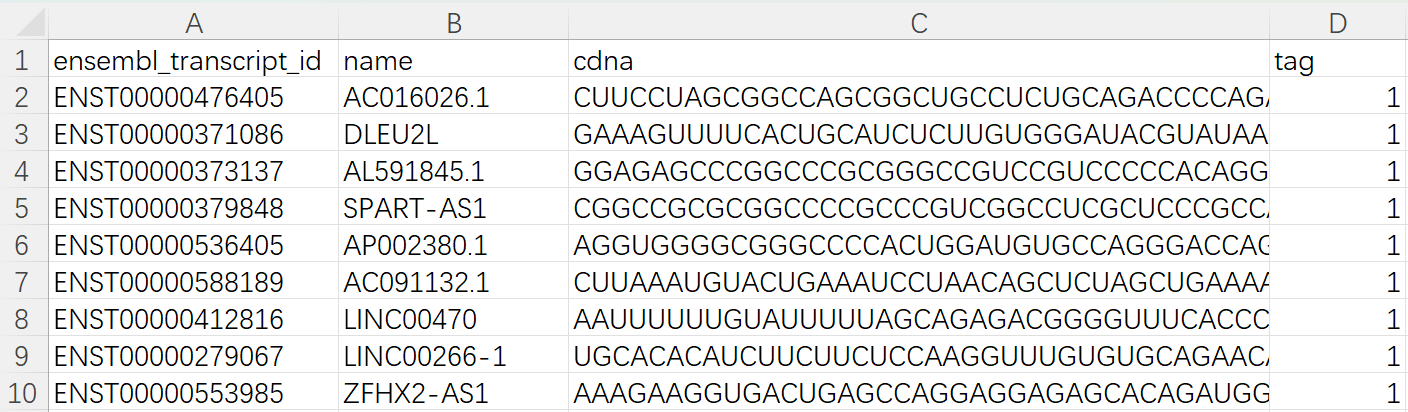
\includegraphics[width=0.8\linewidth]{Figures/数据集展示.png}
        \caption{数据集构成}
        \label{fig:数据集构成}
\end{figure}

\textbf{其中,飞书文档https://sjtu.feishu.cn/docx/KDIjdFXYuoS8a8xbudHc4kpfn1d和ReadMe.md文件记录了实验的所有过程行尝试结果。}

\section{序列表征}


\subsection{K-mer频率方法}

K-mer指的是从基因序列中提取的长度为K的子序列,是一种常用于基因序列分析的概念,广泛应用于基因组学中,尤其是在基因序列的编码、比对和分类任务中,通过将基因序列转换为固定长度的子序列,使得后续的分析更加高效且易于操作。K-mer将一个基因序列按照指定长度K,切分成连续的子序列,每个子序列由K个碱基对(或碱基)组成,并通过不同碱基片段的频率分布来捕捉基因序列中的局部结构特征,从而进行进一步的序列分析。

首先,需要选择K值。较小的K值能够捕捉基因序列中的局部模式,但无法捕捉蕴含更多信息,序列段较长的特征表示,缺乏足够的信息;而较大的K值则能够更好地描述序列的结构特征,减轻重复序列片段的干扰,使模型中的边缘信息增多,但可能导致计算量急剧增加。同时在我们的实验和尝试种,我们发现更大的K值可以是训练更快的收敛,能够更好地描绘训练集中的特征,但也有可能带来更大的过拟合问题。

下一步,我们将针对每一个碱基对序列提取K-mer。以GTAGAGCTGT序列为例,对不同K值,进行K-mers分割运算结果图\ref{fig:K-mers结果示例}所示。

\begin{figure}[h]  
    \centering
    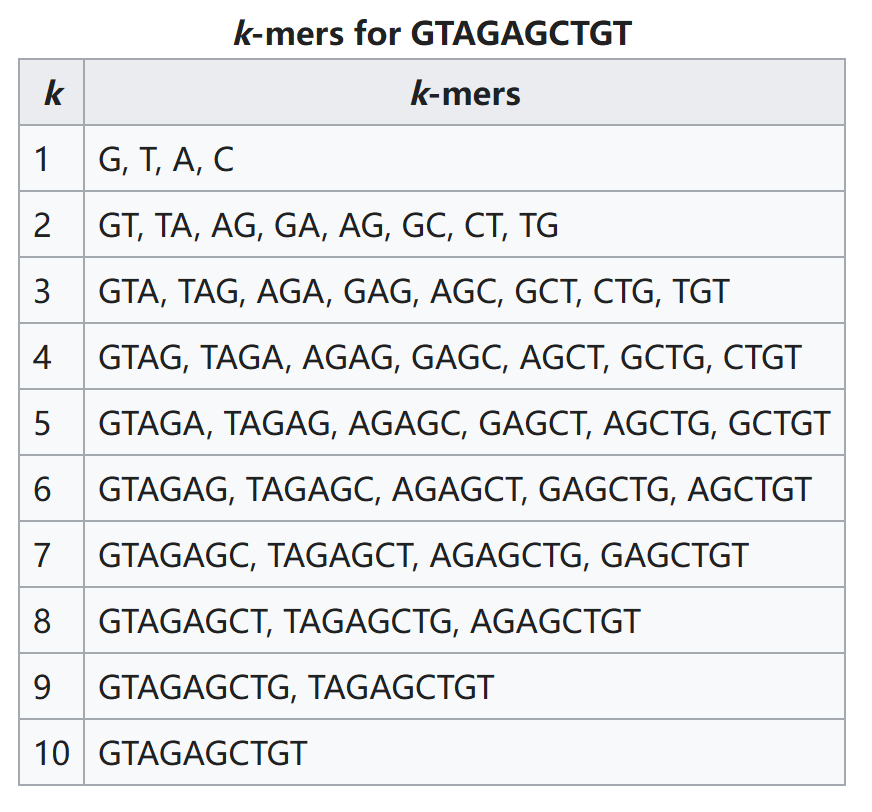
\includegraphics[width=0.6\linewidth]{Figures/K-mers.png}
        \caption{GTAGAGCTGT序列的K-mers结果示例}
        \label{fig:K-mers结果示例}
\end{figure}


第三步,频率统计:在对整个基因组或基因序列进行K-mer分割后,可以统计每个K-mer出现的频率。这些频率向量可以作为基因序列的特征,应用于进一步的分析任务,例如基因分类、序列比对或变异检测。

最后,进行编码表示。在机器学习或数据分析中,K-mer可以被转化为数字特征,用于后续的算法处理。例如,K-mer的频率分布可以被转化为一个向量,表示在一个固定长度的基因序列中,各种K-mer的出现频率。这种方法常用于基因组学中的分类任务或预测任务。

除了编码特征向量,帮助我们的亚细胞定位分类任务,K-mer方法还有广泛应用,包括基因序列比对:通过K-mer,可以快速计算两个基因序列之间的相似度,常用于基因组比对和相似性搜索;变异检测:通过比较K-mer的频率分布,检测基因组中的突变或变异;功能预测:通过对K-mer频率模式的分析,推测基因的功能或对某些疾病的关联等等。

代码中,我们的K-mer方法具体实现如下:
\begin{lstlisting}
def kmer_encoding(sequence, k=3):
    """K-mer频率编码,支持动态k值"""
    kmers = [''.join(x) for x in product('ACGU', repeat=k)]  # 动态生成k-mer组合
    kmer_dict = {kmer: 0 for kmer in kmers}
    
    # 生成K-mer频率向量
    for i in range(len(sequence) - k + 1):
        kmer = sequence[i:i + k]
        if kmer in kmer_dict:
            kmer_dict[kmer] += 1
    
    # 转换为频率
    kmer_freq = np.array(list(kmer_dict.values()))
    return kmer_freq / np.sum(kmer_freq)  # 归一化
\end{lstlisting}


\subsection{RNA-FM方法转化成向量}
\textbf{大作业中用到的RNA-FM方法来源于“Accurate RNA 3D structure prediction using a language model-based deep learning approach”文章中的方法,代码基于https://github.com/ml4bio/RNA-FM。}

RNA-FM(RNA Folding Model)是一个基于深度学习和Transformer架构的模型,主要任务是预测RNA序列的二级结构,其通常由氢键形成的配对关系(如A-U和C-G)来定义。从而,RNA-FM模型能够更高效地捕捉序列中的长距离依赖关系,学习到序列与其对应结构之间的复杂关系。在RNA-FM的训练中,模型通过监督学习方法进行优化,通常使用已经标注了二级结构的RNA序列作为训练数据,并用交叉熵损失等最小化预测结构与真实结构之间的差异,更新其参数。其主要思路架构如图\ref{fig:RNA-FM算法框架}所示。

\begin{figure}[h]  
    \centering
    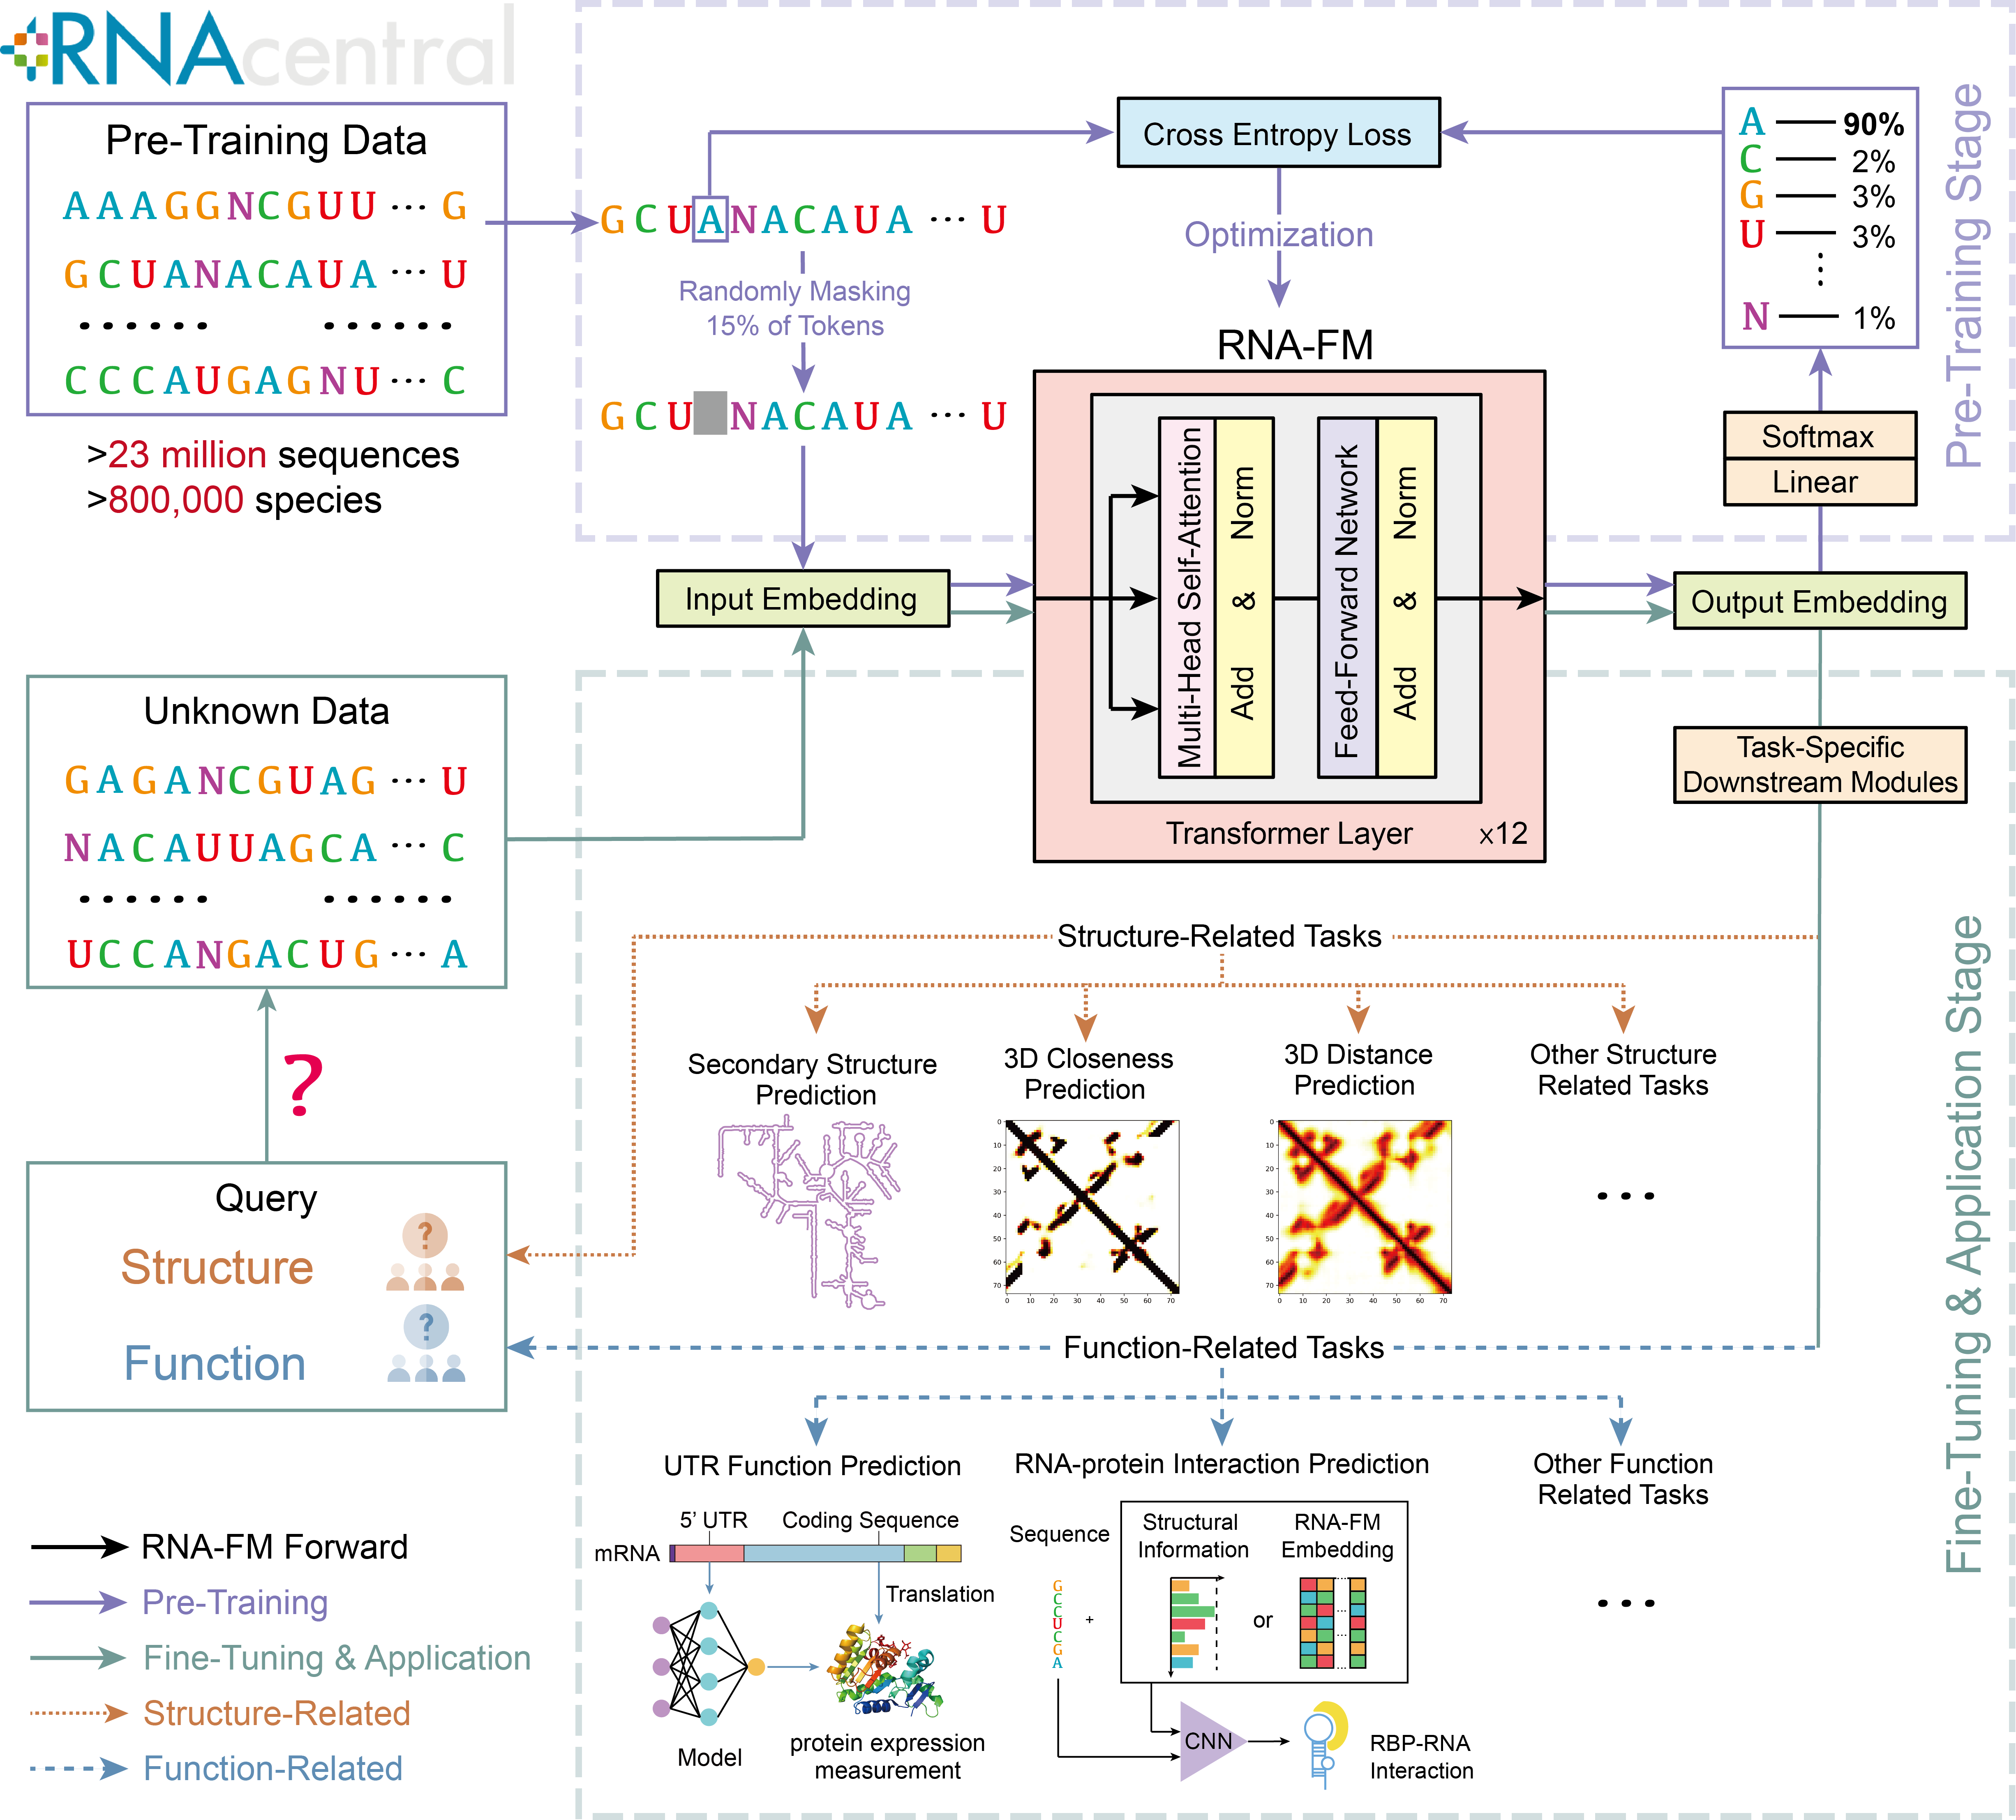
\includegraphics[width=0.8\linewidth]{Figures/RNA-FM.png}
        \caption{FNA-FM算法框架}
        \label{fig:RNA-FM算法框架}
\end{figure}

在RNA-FM中,Transformer架构的关键步骤和实现方式如下。\textbf{第一,}输入嵌入层。RNA序列首先经过一个嵌入层,将每个碱基(A、U、G、C)转换为一个稠密的向量表示。\textbf{第二,}自注意力机制(Self-Attention)。序列的每一个碱基(位置)通过自注意力层,考虑与其他碱基之间的相互关系,因为RNA的二级结构往往由远距离的碱基对组成,需要自注意力来捕捉这些远距离的相互作用。\textbf{第三,}多头注意力(Multi-Head Attention)。将自注意力分成多个“头”,每个头独立计算注意力权重,捕捉不同的特征或关系。RNA-FM利用该机制并行处理多个不同的依赖关系,增强模型的表达能力,使其能够同时考虑不同的结构特征。\textbf{第四,}位置编码(Positional Encoding)。Transformer架构本身不具备处理序列顺序的能力,因此需要位置编码来提供关于序列中各个位置的信息。RNA-FM利用位置编码来表示RNA序列中每个碱基的位置,从而让模型理解序列的结构和顺序。\textbf{第五,}前馈网络(Feed-Forward Networks)。前馈神经网络对提取的特征进行进一步处理,帮助模型从自注意力层中学到的高维特征中进行降维,并提取重要信息。\textbf{第六,}解码层(Decoder)。RNA-FM利用解码层将模型输出的特征映射到RNA的二级结构。这个过程涉及将RNA的序列信息转换为结构信息,包括预测哪些碱基是配对的。其模型架构如\ref{}所示。

\begin{figure}[h]  
    \centering
    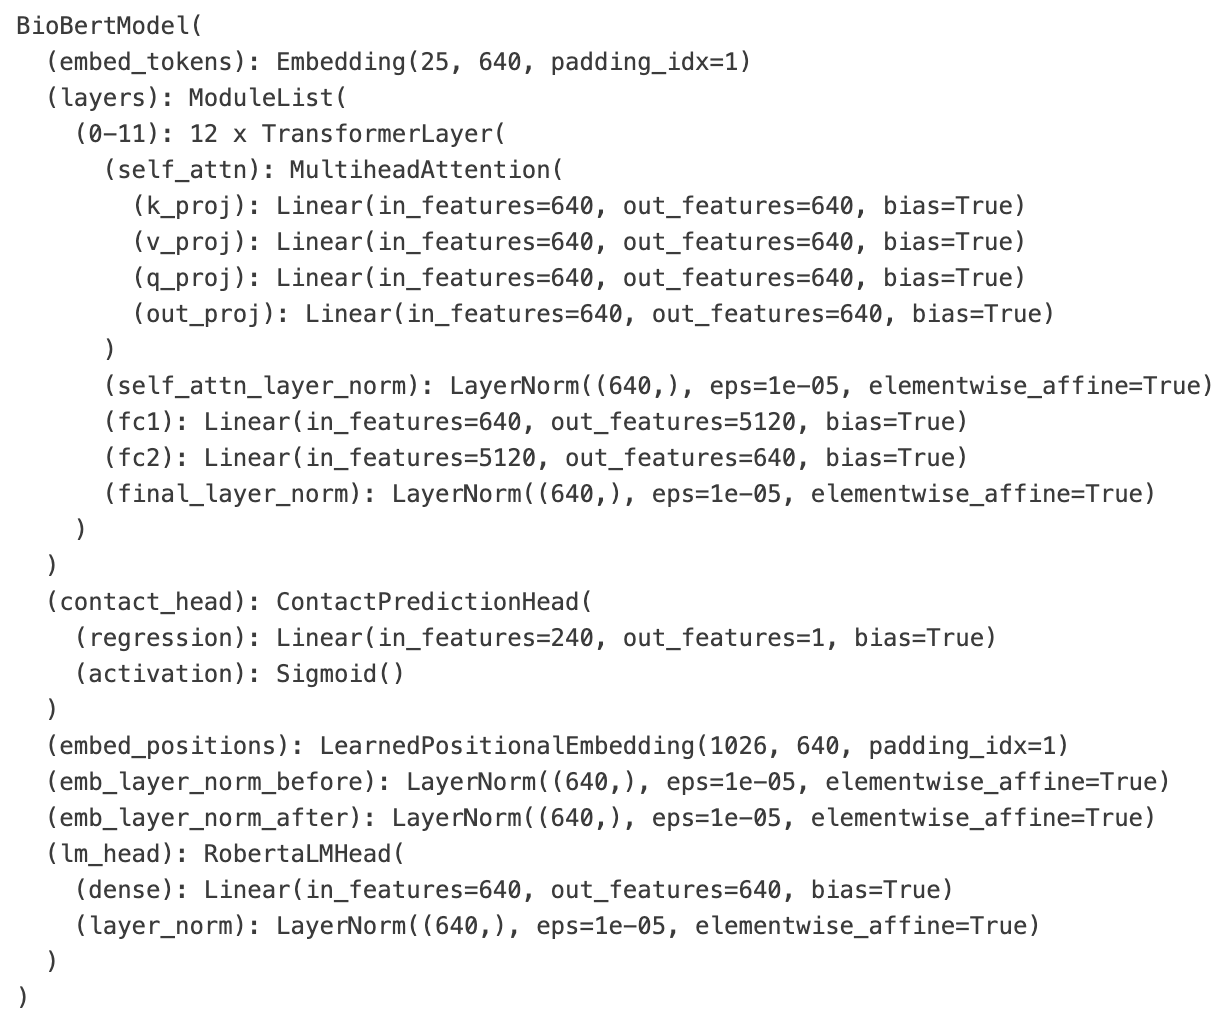
\includegraphics[width=0.8\linewidth]{Figures/model_structure.jpg
    }
        \caption{Transformer模型架构}
        \label{fig:Transformer模型架构}
\end{figure}

使用其预训练好的模型对我们数据进行编码的主要代码如下:

\begin{lstlisting}
# Load RNA-FM model
fm_model, alphabet  = fm.pretrained.rna_fm_t12("RNA-FM_pretrained.pth") 
batch_converter = alphabet.get_batch_converter()
fm_model.to(device)

fm_model.eval()  # disables dropout for deterministic results

chunk_size = 10

# pre-allocate the space to save memory
torch.cuda.empty_cache()
token_embeddings = np.zeros((len(labels), 1024, 640))
torch.cuda.empty_cache()
# divide all the sequences into chunks for processing due to the GPU memory limit
for i in tqdm(range(0, len(seqs), chunk_size), desc=f'Processing chunks'):
    data = seqs[i:i+chunk_size]
    batch_labels, batch_strs, batch_tokens = batch_converter(data)

    # use GPU
    with torch.no_grad():
        results = fm_model(batch_tokens.to(device), repr_layers=[12])

    emb = results["representations"][12].cpu().numpy()
    token_embeddings[i:i+chunk_size, :emb.shape[1], :] = emb
    torch.cuda.empty_cache()
\end{lstlisting}

后面,与戚治齐同学一同讨论,基于github上的代码基础框架,通过Transformer编码得到的结果,以及一个较为简单的神经分类网络,初步尝试并不令人满意。如图\ref{fig:RNAFM_results}所示,随着train loss的逐渐下降,val loss处于一个波动走高的趋势,模型展现出过拟合的倾向,泛化性不好。从准确度角度看,train accuracy和test accuracy本身的值都不高,随着train accuracy的逐渐上升,test accuracy逐渐下降,两者都展现出了很强烈的波动性,模型分类的稳定性不好。

\begin{figure}[h]
    \centering
    \begin{minipage}{0.49\linewidth}
        \centering
        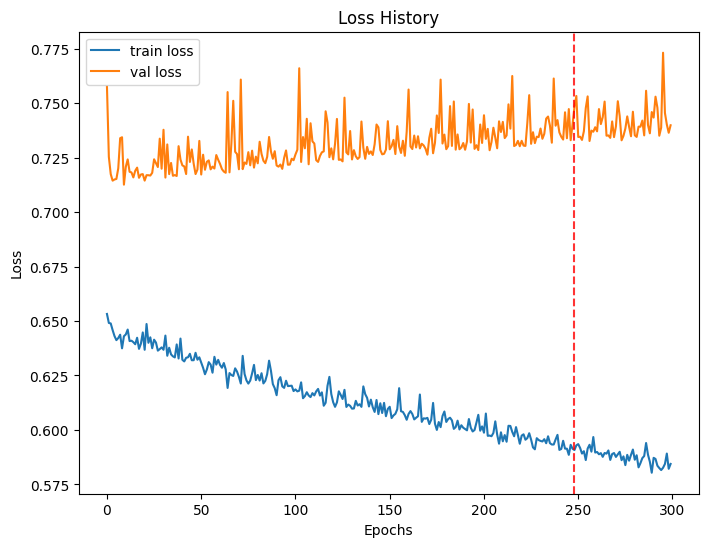
\includegraphics[height=0.67\linewidth]{Figures/RNAFM_loss.png}
        \caption*{(a) RNA-FM方法loss结果}
    \end{minipage}
    % \hfill % 添加空白填充,确保图片之间有一些间隔
    \begin{minipage}{0.49\linewidth}
        \centering
        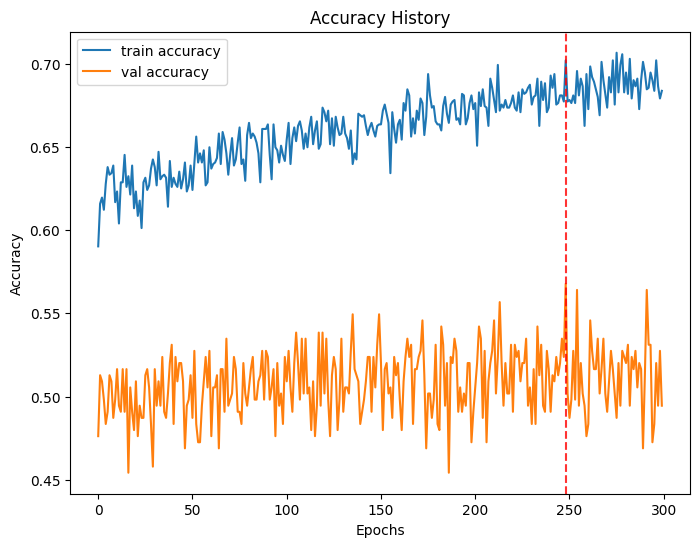
\includegraphics[height=0.67\linewidth]{Figures/RNAFM_acc.png}
        \caption*{(b) RNA-FM方法accuracy结果}
    \end{minipage}
    \caption{RNA-FM方法结果}
    \label{fig:RNAFM_results}
\end{figure}

此外,实验中还发现,增加神经网络的复杂程度并不能很好地增强预测和分类的准确度,说明并不是网络的复杂程度不够高,可能在编码效果上出了一些问题。同时,在Transformer的编码训练中,我们只采用了40\%的数据集以提升模型在电脑上的运行效率,这种做法可能对生物信息学数据集的完整性产生了较大的影响,导致编码效果不佳。所以,接下来我将从K-mer编码入手,通过更具有可解释性的方法,提取RNA序列的特征,并比较其响应参数和方法的差异和效果。


\section{神经网络 Neural Network}

\subsection{网络框架搭建}
在训练的一开始,我们意识到在加载数据,划分数据集,以及神经网络的训练过程中,会引入随机性。因此,首先需要选定控制整个代码框架的随机种子,确保实验结果可复现。随机种子的设置函数如下所示:
\begin{lstlisting}
def set_seed(seed=42):
    np.random.seed(seed)
    random.seed(seed)
    torch.manual_seed(seed)
    torch.cuda.manual_seed_all(seed)
\end{lstlisting}

经过多次尝试,本任务对神经网络架构的总体复杂程度要求不是非常高,网络结构的复杂程度对最终的training accuracy, validation accuracy 和 test accuracy没有起到显著影响,其主要差异可能还是体现在需要的神经元数量以及收敛速度等方面。我们主要定义了三种不同的神经网络架构,包括RNA\_Classifier,RNA\_Classifier\_2以及RNA\_Classifier\_3,其具体定义和前向传播函数如下:

\begin{lstlisting}
    class RNA_Classifier(nn.Module):
    def __init__(self, input_size, hidden_size):
        super(RNA_Classifier, self).__init__()
        self.fc1 = nn.Linear(input_size, hidden_size)
        self.fc2 = nn.Linear(hidden_size, 1)
        self.sigmoid = nn.Sigmoid()

    def forward(self, x):
        x = torch.relu(self.fc1(x))
        x = self.fc2(x)
        return self.sigmoid(x)


class RNA_Classifier_2(nn.Module):
    def __init__(self, input_size, hidden_size, dropout_prob=0.5):
        super(RNA_Classifier_2, self).__init__()
        
        # 定义网络结构
        self.fc1 = nn.Linear(input_size, hidden_size)  # 第一层全连接
        self.batchnorm1 = nn.BatchNorm1d(hidden_size)  # 第一层 BatchNorm
        self.dropout1 = nn.Dropout(p=dropout_prob)    # 第一层 Dropout
        
        self.fc2 = nn.Linear(hidden_size, 1)          # 第二层全连接
        self.sigmoid = nn.Sigmoid()                  # 输出层激活函数

    def forward(self, x):
        # 前向传播
        x = self.fc1(x)                              # 第一层全连接
        x = self.batchnorm1(x)                       # 第一层 BatchNorm
        x = torch.relu(x)                            # 激活函数 ReLU
        x = self.dropout1(x)                         # 第一层 Dropout
        
        x = self.fc2(x)                              # 第二层全连接
        return self.sigmoid(x)                       # 输出层激活


# 定义神经网络模型
class RNA_Classifier_3(nn.Module):
    def __init__(self, input_size, hidden_size=128, dropout_rate=0.5):
        super(RNA_Classifier_3, self).__init__()
        self.fc1 = nn.Linear(input_size, hidden_size)
        self.fc2 = nn.Linear(hidden_size, hidden_size)
        self.fc3 = nn.Linear(hidden_size, hidden_size)
        self.fc4 = nn.Linear(hidden_size, 1)
        self.relu = nn.ReLU()
        self.sigmoid = nn.Sigmoid()
        self.dropout = nn.Dropout(dropout_rate)
        
    def forward(self, x):
        x = self.fc1(x)
        x = self.relu(x)
        x = self.fc2(x)
        x = self.relu(x)
        x = self.fc3(x)
        x = self.relu(x)
        x = self.dropout(x)
        x = self.fc4(x)
        x = self.sigmoid(x)
        return x
\end{lstlisting}

三个网络在结构上逐渐复杂,但仍有不少共同的元素,下面分析这三个模型的共同层及其作用、二分类的实现方式、引入非线性的激活函数,以及它们之间的递进功能区别。

\textbf{首先,全连接层}(Fully Connected Layers, 'nn.Linear')。全连接层是最基本的神经网络层之一,它将输入的每一个神经元与输出的每一个神经元进行线性组合。具体来说,'nn.Linear(input\_size, output\_size)'定义了一个线性变换:$y = xw^T + b$,其中 $w$ 是权重矩阵,$b$ 是偏置向量。在这三个模型中,全连接层用于将输入特征映射到隐藏表示,逐步提取和转换特征,以适应分类任务的需求。'RNA\_Classifier'包含两层全连接层,fc1和fc2。'RNA\_Classifier\_2'同样包含两层全连接层,但增加了 Batch Normalization 和 Dropout。'RNA\_Classifier\_3'包含四层全连接层,fc1,fc2,fc3和fc4以构建更深的网络结构。

\textbf{其次,激活函数}(Activation Functions),在本次网络的设计中主要采用ReLU和Sigmoid。ReLU(Rectified Linear Unit)是常用的非线性激活函数,定义为 $f(x) = \max(0, x)$。它引入了非线性,使得神经网络能够学习复杂的函数映射,同时计算效率高,缓解了梯度消失问题。而Sigmoid 函数将输入压缩到(0, 1)的区间,常用于二分类任务的输出层,以输出概率值。三个模型在最后一层都使用 Sigmoid 激活函数,将网络的输出转换为概率,用于二分类。

\textbf{第三,批归一化},Batch Normalization ('nn.BatchNorm1d)。在Batch Normalization 对每一批次的数据进行标准化,减少内部协变量偏移,加速训练过程,提高模型的稳定性和性能。在 'RNA\_Classifier\_2' 中尝试在第一层全连接层之后应用 Batch Normalization,使得输出分布更加稳定,促进更有效的学习,观察是否对模型的训练有较大提升。

\textbf{第四,Dropout} ('nn.Dropout')'RNA\_Classifier\_2'和 'RNA\_Classifier\_3' 中使用)Dropout 这种正则化技术,通过在训练过程中随机丢弃一部分神经元,防止过拟合,增强模型的泛化能力。
   
在接下来的二分类的实现方式中,三个模型的结构相同。在输出层,最后一层全连接层的输出维度为 1,表示单一的输出值,用于二分类。使用 Sigmoid 激活函数将输出值压缩到 `(0, 1)` 之间,表示为类别 1 的概率。使用 'nn.BCELoss',根据 Sigmoid 输出的概率值,与实际标签计算二分类的损失。

非线性成分的引入也是通过ReLU 激活函数和Sigmoid激活函数,在隐藏层引入非线性,使得模型能够学习复杂的非线性关系;在输出层引入非线性,将线性输出转化为概率值,适用于二分类任务。

'RNA\_Classifier'使用两层全连接层,适用于较为简单的二分类任务,没有正则化手段(如 BatchNorm 和 Dropout)。'RNA\_Classifier\_2'也是两层全连接层,增加了 Batch Normalization 和 Dropout,增强训练的稳定性和加速收敛,同时使用 Dropout,防止过拟合,提高模型的泛化能力。'RNA\_Classifier\_3'使用四层全连接层(更深的网络结构),包括三个隐藏层和一个输出层,含有多个 ReLU 激活函数,增强模型的非线性表达能力。



\subsection{模型训练}

整个的训练过程定义在train.py文件中的classification函数中,其中训练数据集的路径,测试数据集的路径,K-mer的k参数选择,隐层的神经元数量规模,batch\_size的大小,训练轮数和选择的网络架构,在被主函数调用时,均都通过args方法从命令行中传入,提升了实验测试时参数调整的效率。函数的具体实现过程见附录。

\begin{lstlisting}
def classification(training_file, test_file, k=3, hidden_size=128, batch_size=32, epochs=20, network='RNA_Classifier'):
\end{lstlisting}

整个分类流程首先读取训练和测试数据文件,并从中提取RNA序列及其对应的标签。接着,利用K-mer编码将RNA序列转换为数值特征向量,并对这些特征进行标准化处理,以确保数据具有均匀的分布。随后,将训练数据进一步划分为训练集和验证集,同时保持标签分布的一致性,也即是分层采样。接下来,将处理后的数据转换为适用于PyTorch的张量格式,以便于在神经网络中使用。根据在命令行中传入的网络类型,初始化相应的神经网络模型,并定义二分类任务的损失函数(如二元交叉熵损失)和优化器(如Adam)。在训练阶段,模型在多个训练轮次中逐批处理训练数据,通过前向传播计算输出,反向传播更新模型参数,并记录每个轮次的训练损失和准确率。每完成一个轮次后,使用验证集评估模型的性能,记录验证损失和准确率。训练完成后,最终在测试集上评估模型的准确率,以验证模型的泛化能力。整个流程涵盖了数据预处理、模型选择与初始化、训练与验证、以及最终的测试评估,确保从原始RNA序列到二分类结果的完整实现。


\subsection{网络架构比较}

我们固定其他参数不变,取hidden\_size为330,采用2-Mer编码,在训练轮数epoch为40和200的情况下分别测试其预测效果,如表\ref{tab:CNN方法网络架构比较}和图\ref{fig:RNA-Regression Compare},图\ref{fig:RNA-Regression-2 Compare},图\ref{fig:RNA-Regression-3 Compare}所示。

\begin{table*}[h]
\centering
\footnotesize
\setlength{\tabcolsep}{5pt}
\caption{NN方法网络架构比较}
\label{tab:CNN方法网络架构比较}
{
    \begin{tabular}{cccccc}
    \toprule
    \textbf{Model(epochs)} & \textbf{Train\_Loss}($\downarrow$) & \textbf{Val\_Loss}($\downarrow$)  & \textbf{Train\_Accuracy\%}($\uparrow$)  & \textbf{Val\_accuracy\%}($\uparrow$)  & \textbf{Test\_Accuracy\%}($\uparrow$)
    \\
    \midrule
    RNA\_Classifier(40) & 0.0187 & 0.5940 & 67.50 & 69.11 & 69.74\\
    RNA\_Classifier\_2(40) & 0.0196 & 0.5929 & 65.34 & 69.11 & 69.74\\
    RNA\_Classifier\_3(40) & 0.0148 & 0.6430 & 77.98 & 66.91 & 69.21\\
    RNA\_Classifier(200) & 0.0178 & 0.6009 & 69.33 & 67.50 & 69.74\\
    RNA\_Classifier\_2(200) & 0.0185 & 0.5936 & 69.22 & 68.81 & 71.05\\
    RNA\_Classifier\_3(200) & 0.0008 & 2.8505 & 99.27 & 61.93 & 64.74\\
    \bottomrule
    \end{tabular}
}
\end{table*}

\begin{figure}[h]
    \centering
    \begin{minipage}{0.49\linewidth}
        \centering
        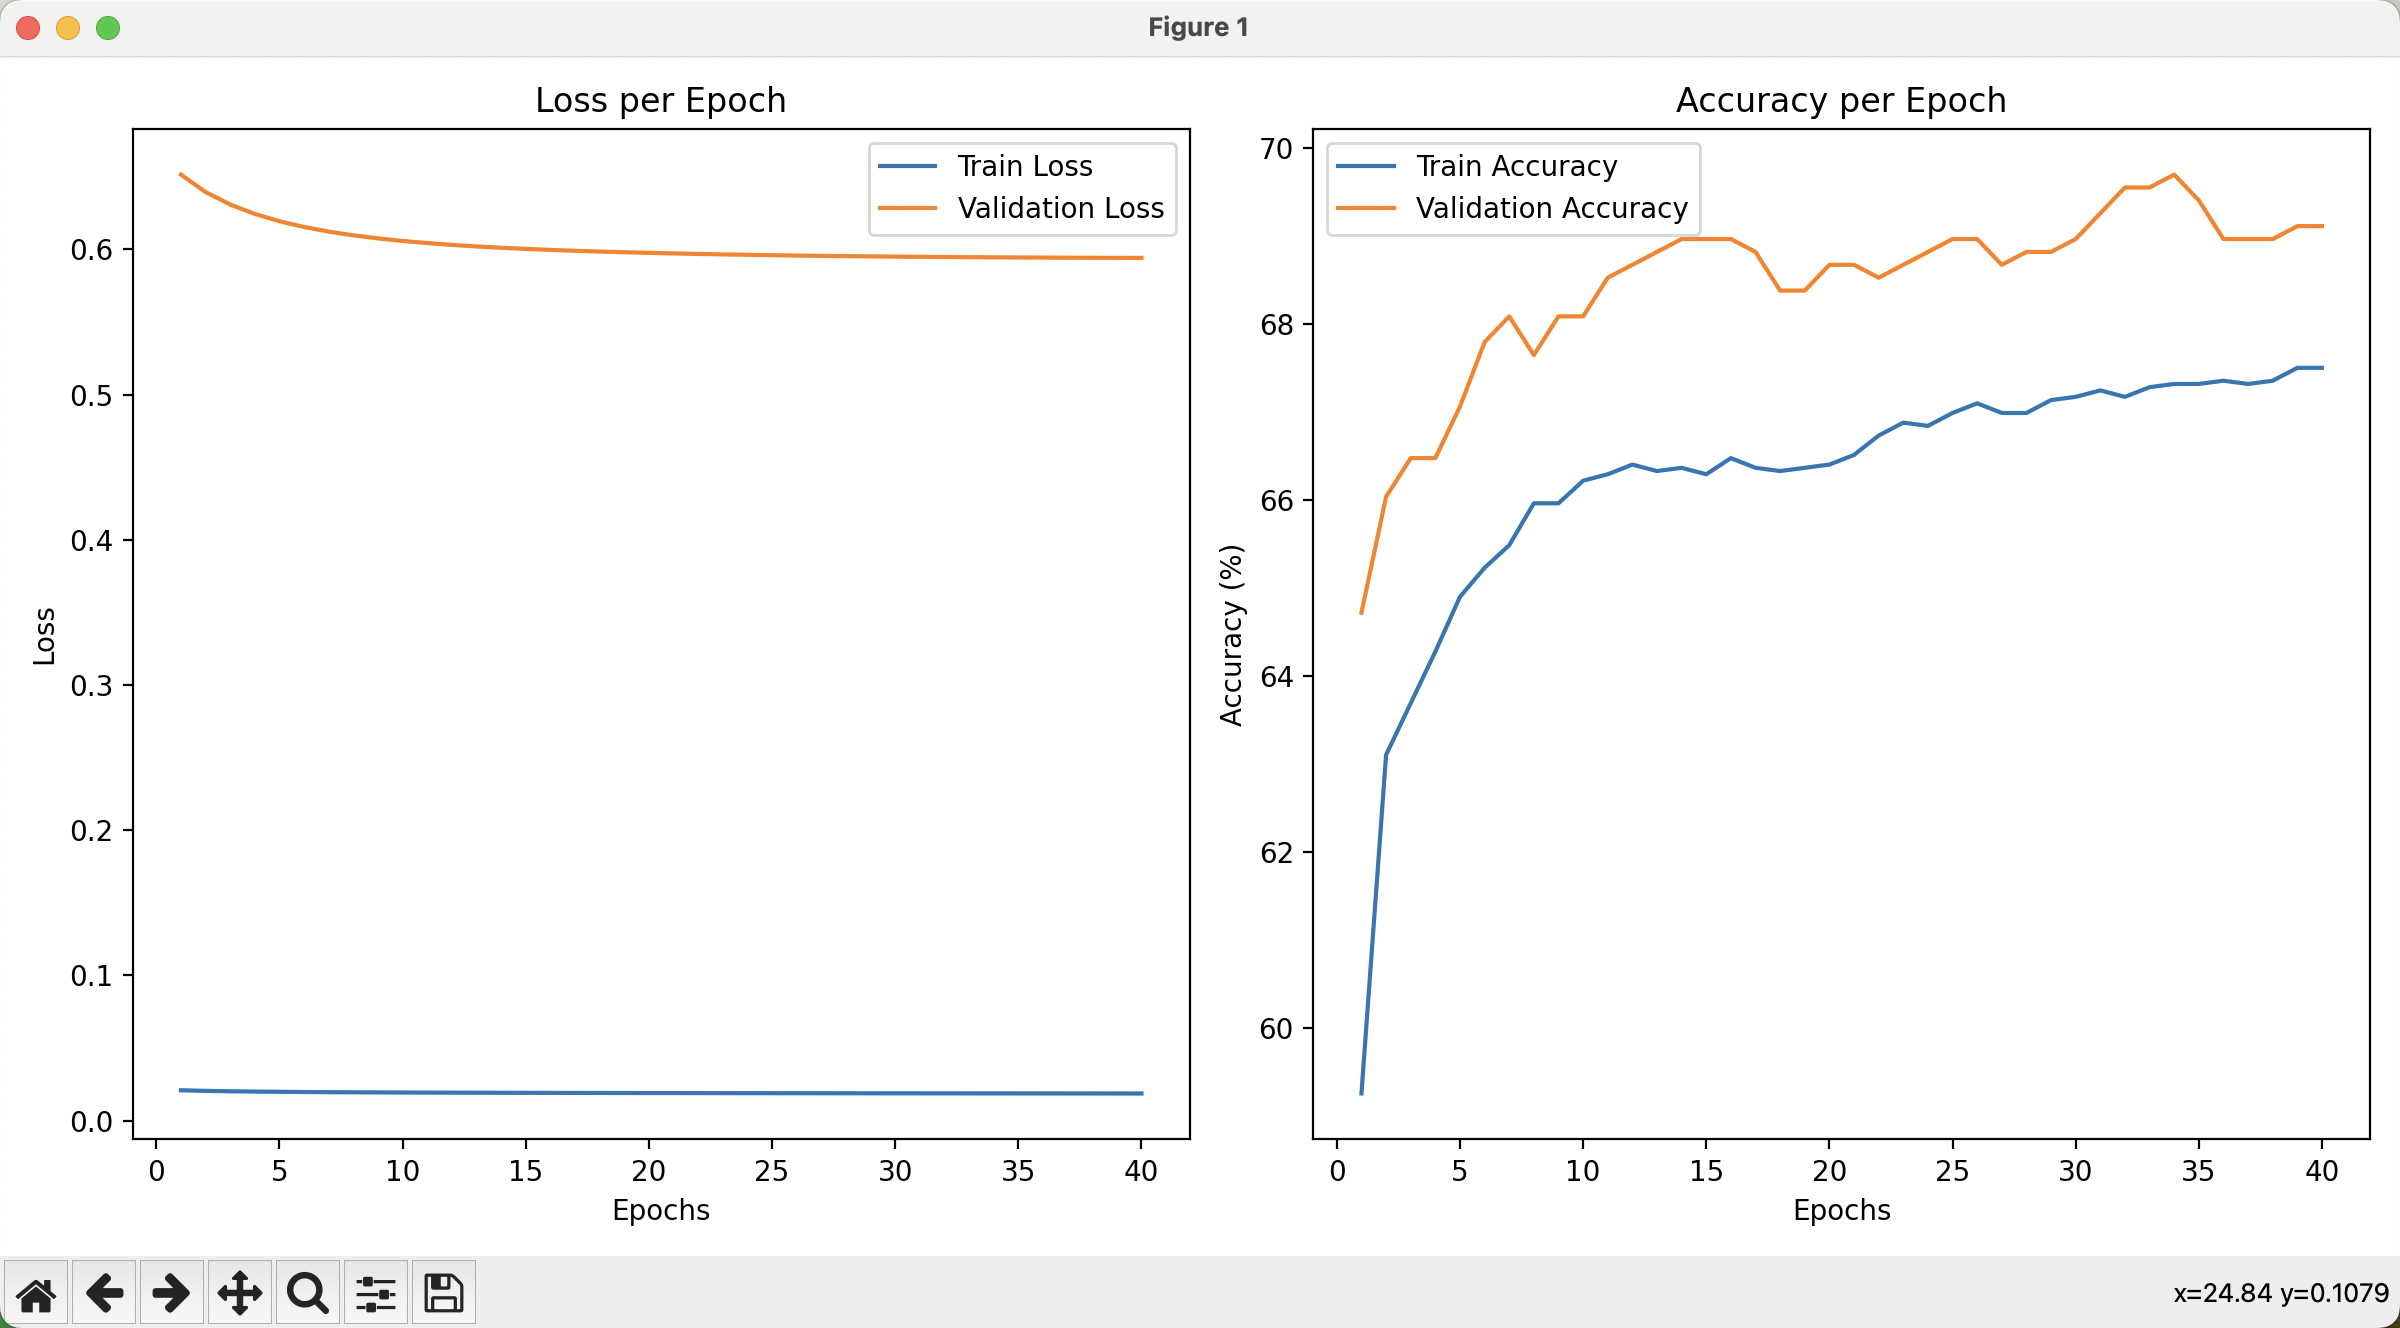
\includegraphics[height=0.55\linewidth]{Figures/1-40.png}
        \caption*{(a) 40 epoch}
    \end{minipage}
    % \hfill % 添加空白填充,确保图片之间有一些间隔
    \begin{minipage}{0.49\linewidth}
        \centering
        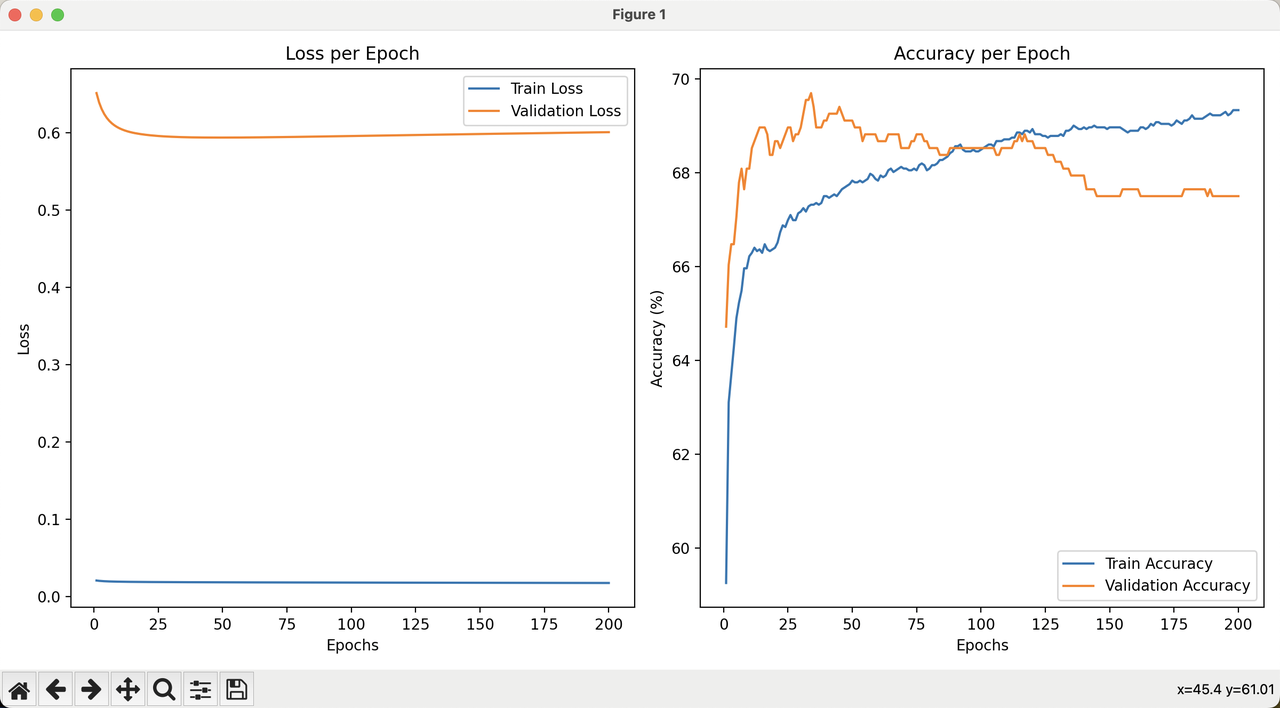
\includegraphics[height=0.55\linewidth]{Figures/1-200.png}
        \caption*{(b) 200 epoch}
    \end{minipage}
    \caption{RNA\_Regression模型结果比较}
    \label{fig:RNA-Regression Compare}
\end{figure}

\begin{figure}[h]
    \centering
    \begin{minipage}{0.49\linewidth}
        \centering
        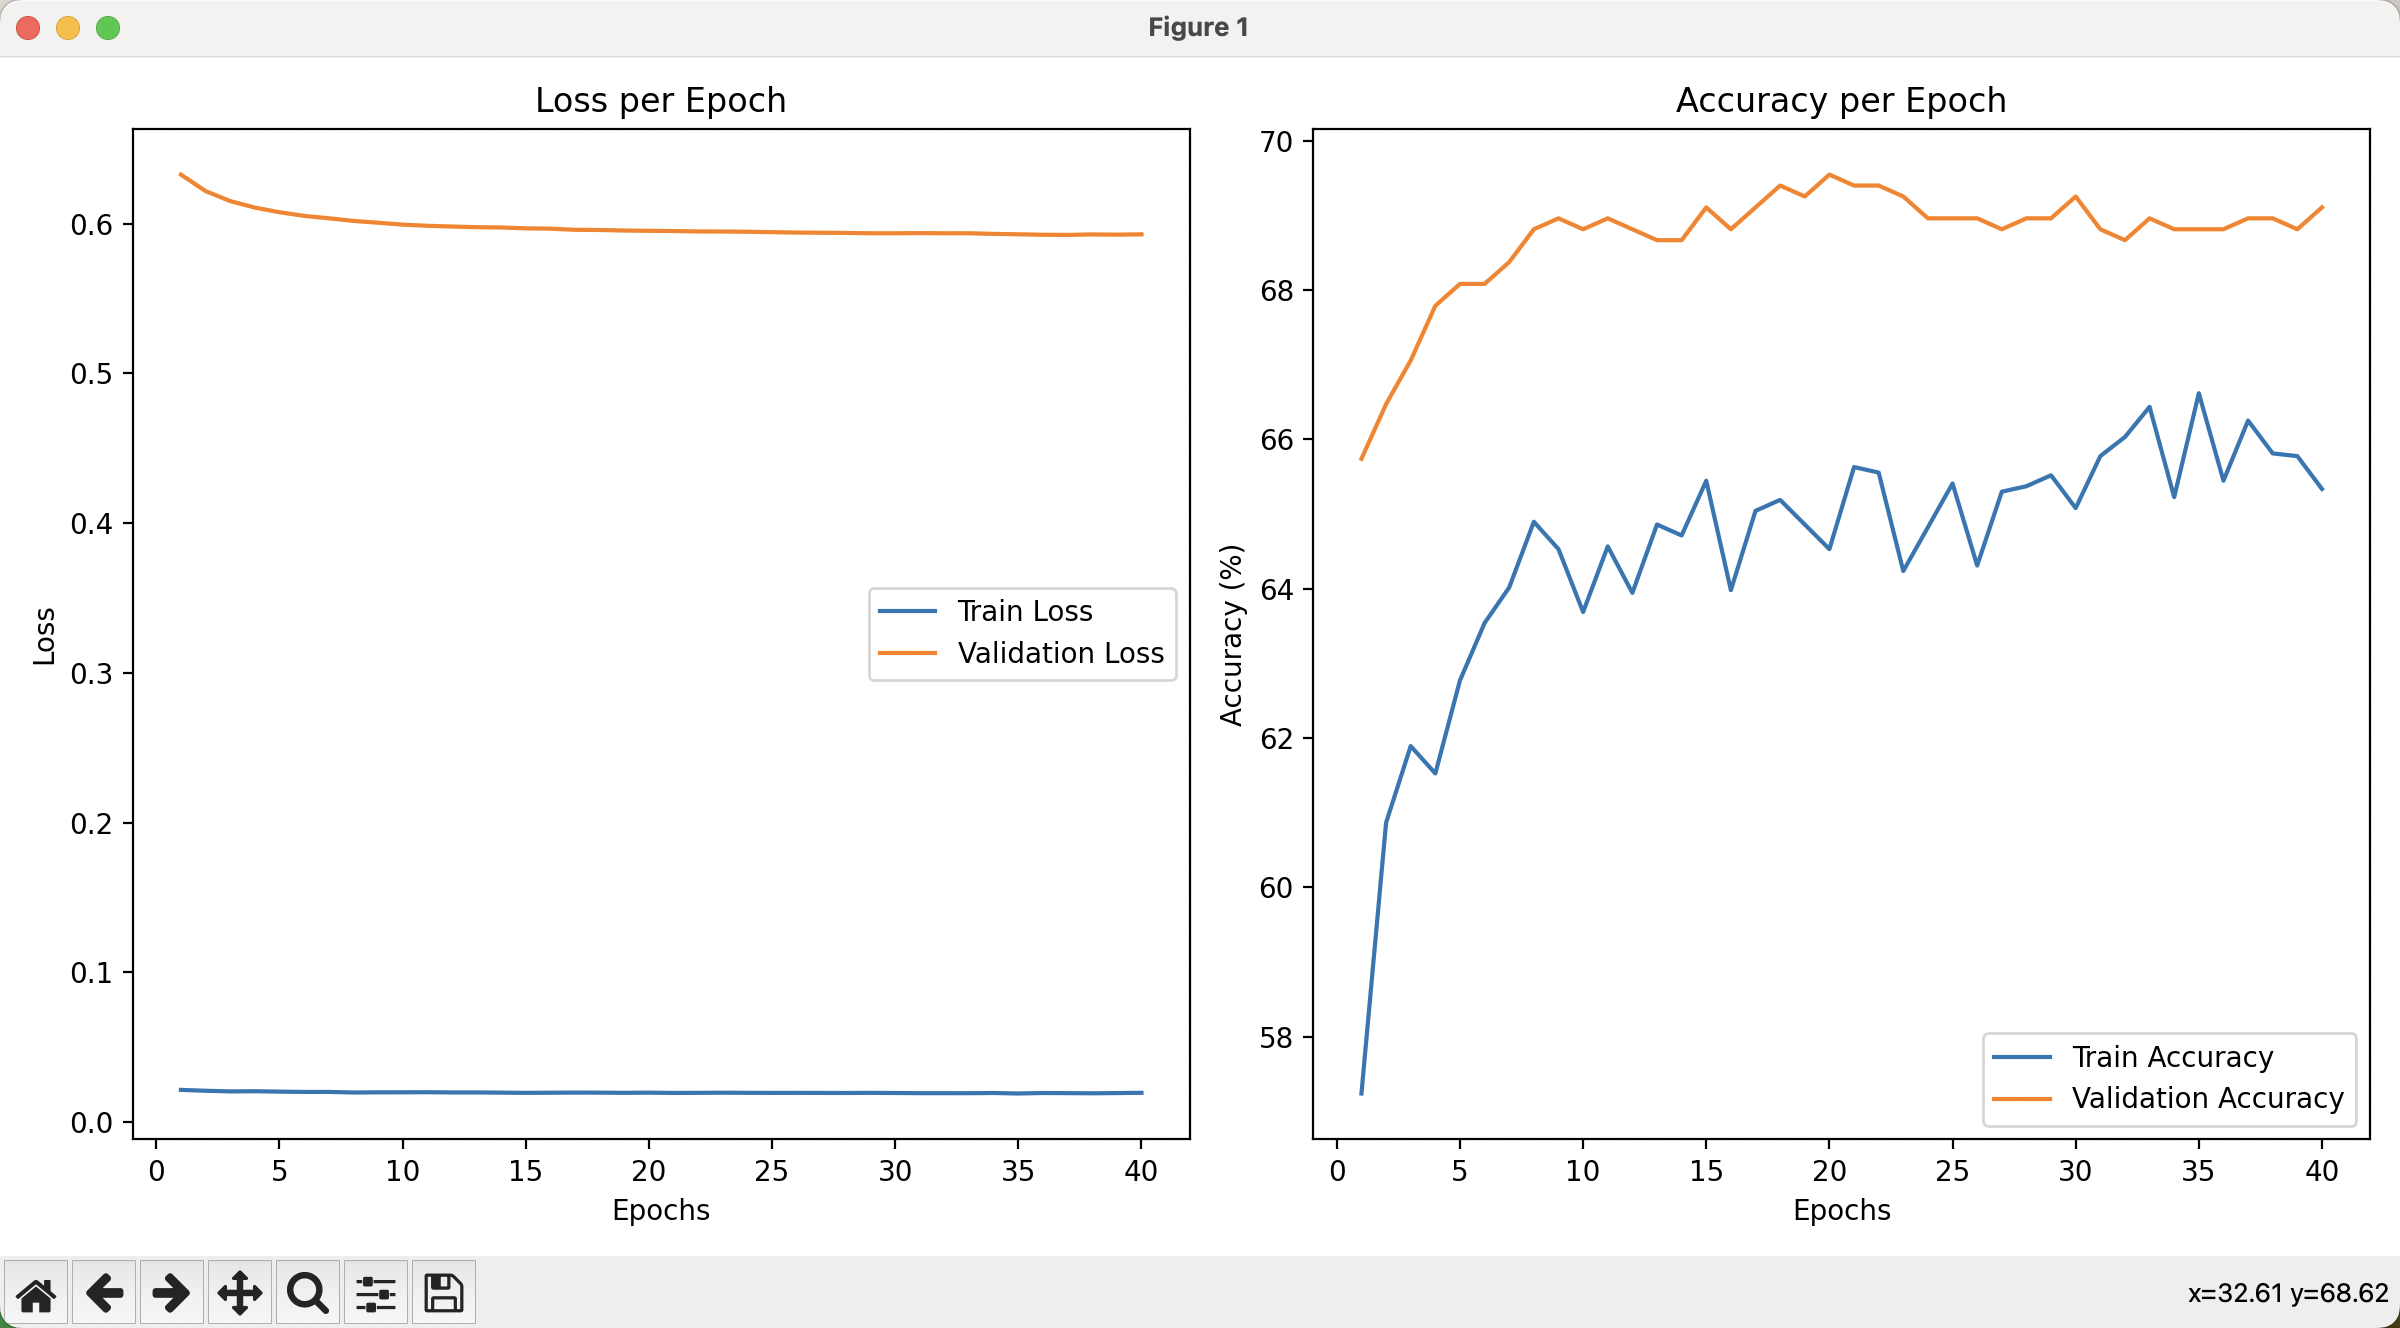
\includegraphics[height=0.55\linewidth]{Figures/2-40.png}
        \caption*{(a) 40 epoch}
    \end{minipage}
    % \hfill % 添加空白填充,确保图片之间有一些间隔
    \begin{minipage}{0.49\linewidth}
        \centering
        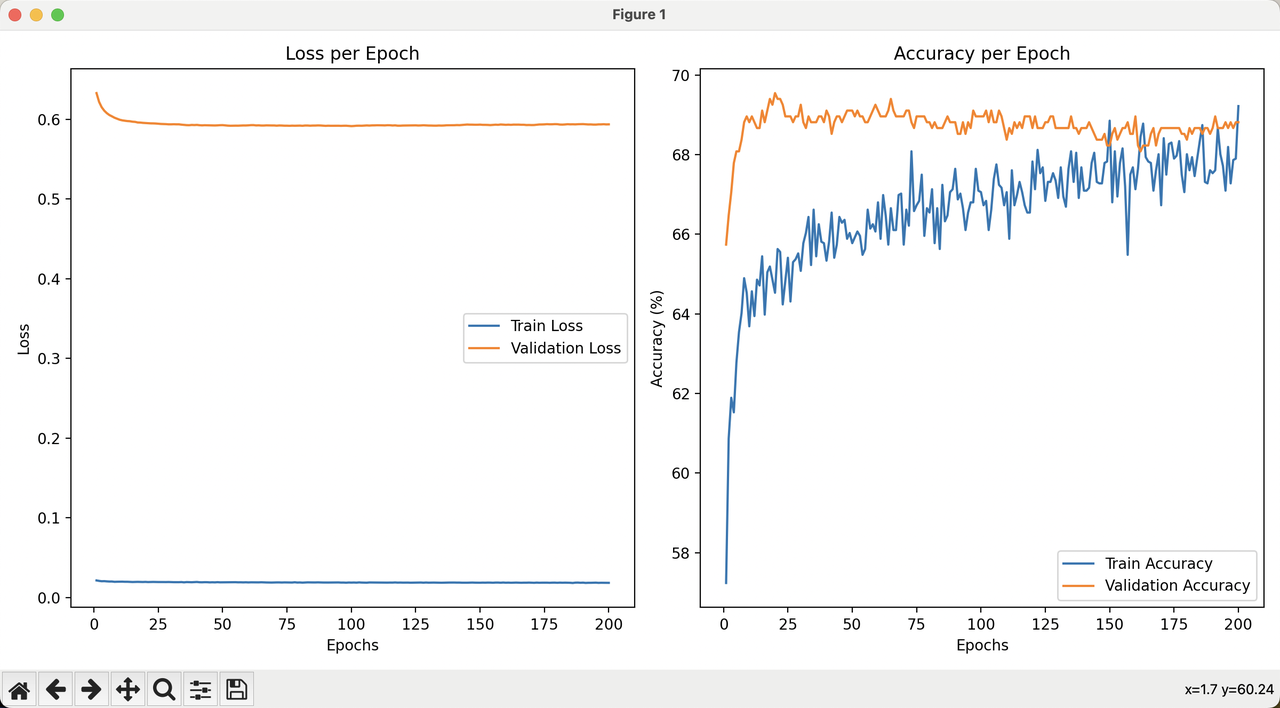
\includegraphics[height=0.55\linewidth]{Figures/2-200.png}
        \caption*{(b) 200 epoch}
    \end{minipage}
    \caption{RNA\_Regression\_2模型结果比较}
    \label{fig:RNA-Regression-2 Compare}
\end{figure}

\begin{figure}[h]
    \centering
    \begin{minipage}{0.49\linewidth}
        \centering
        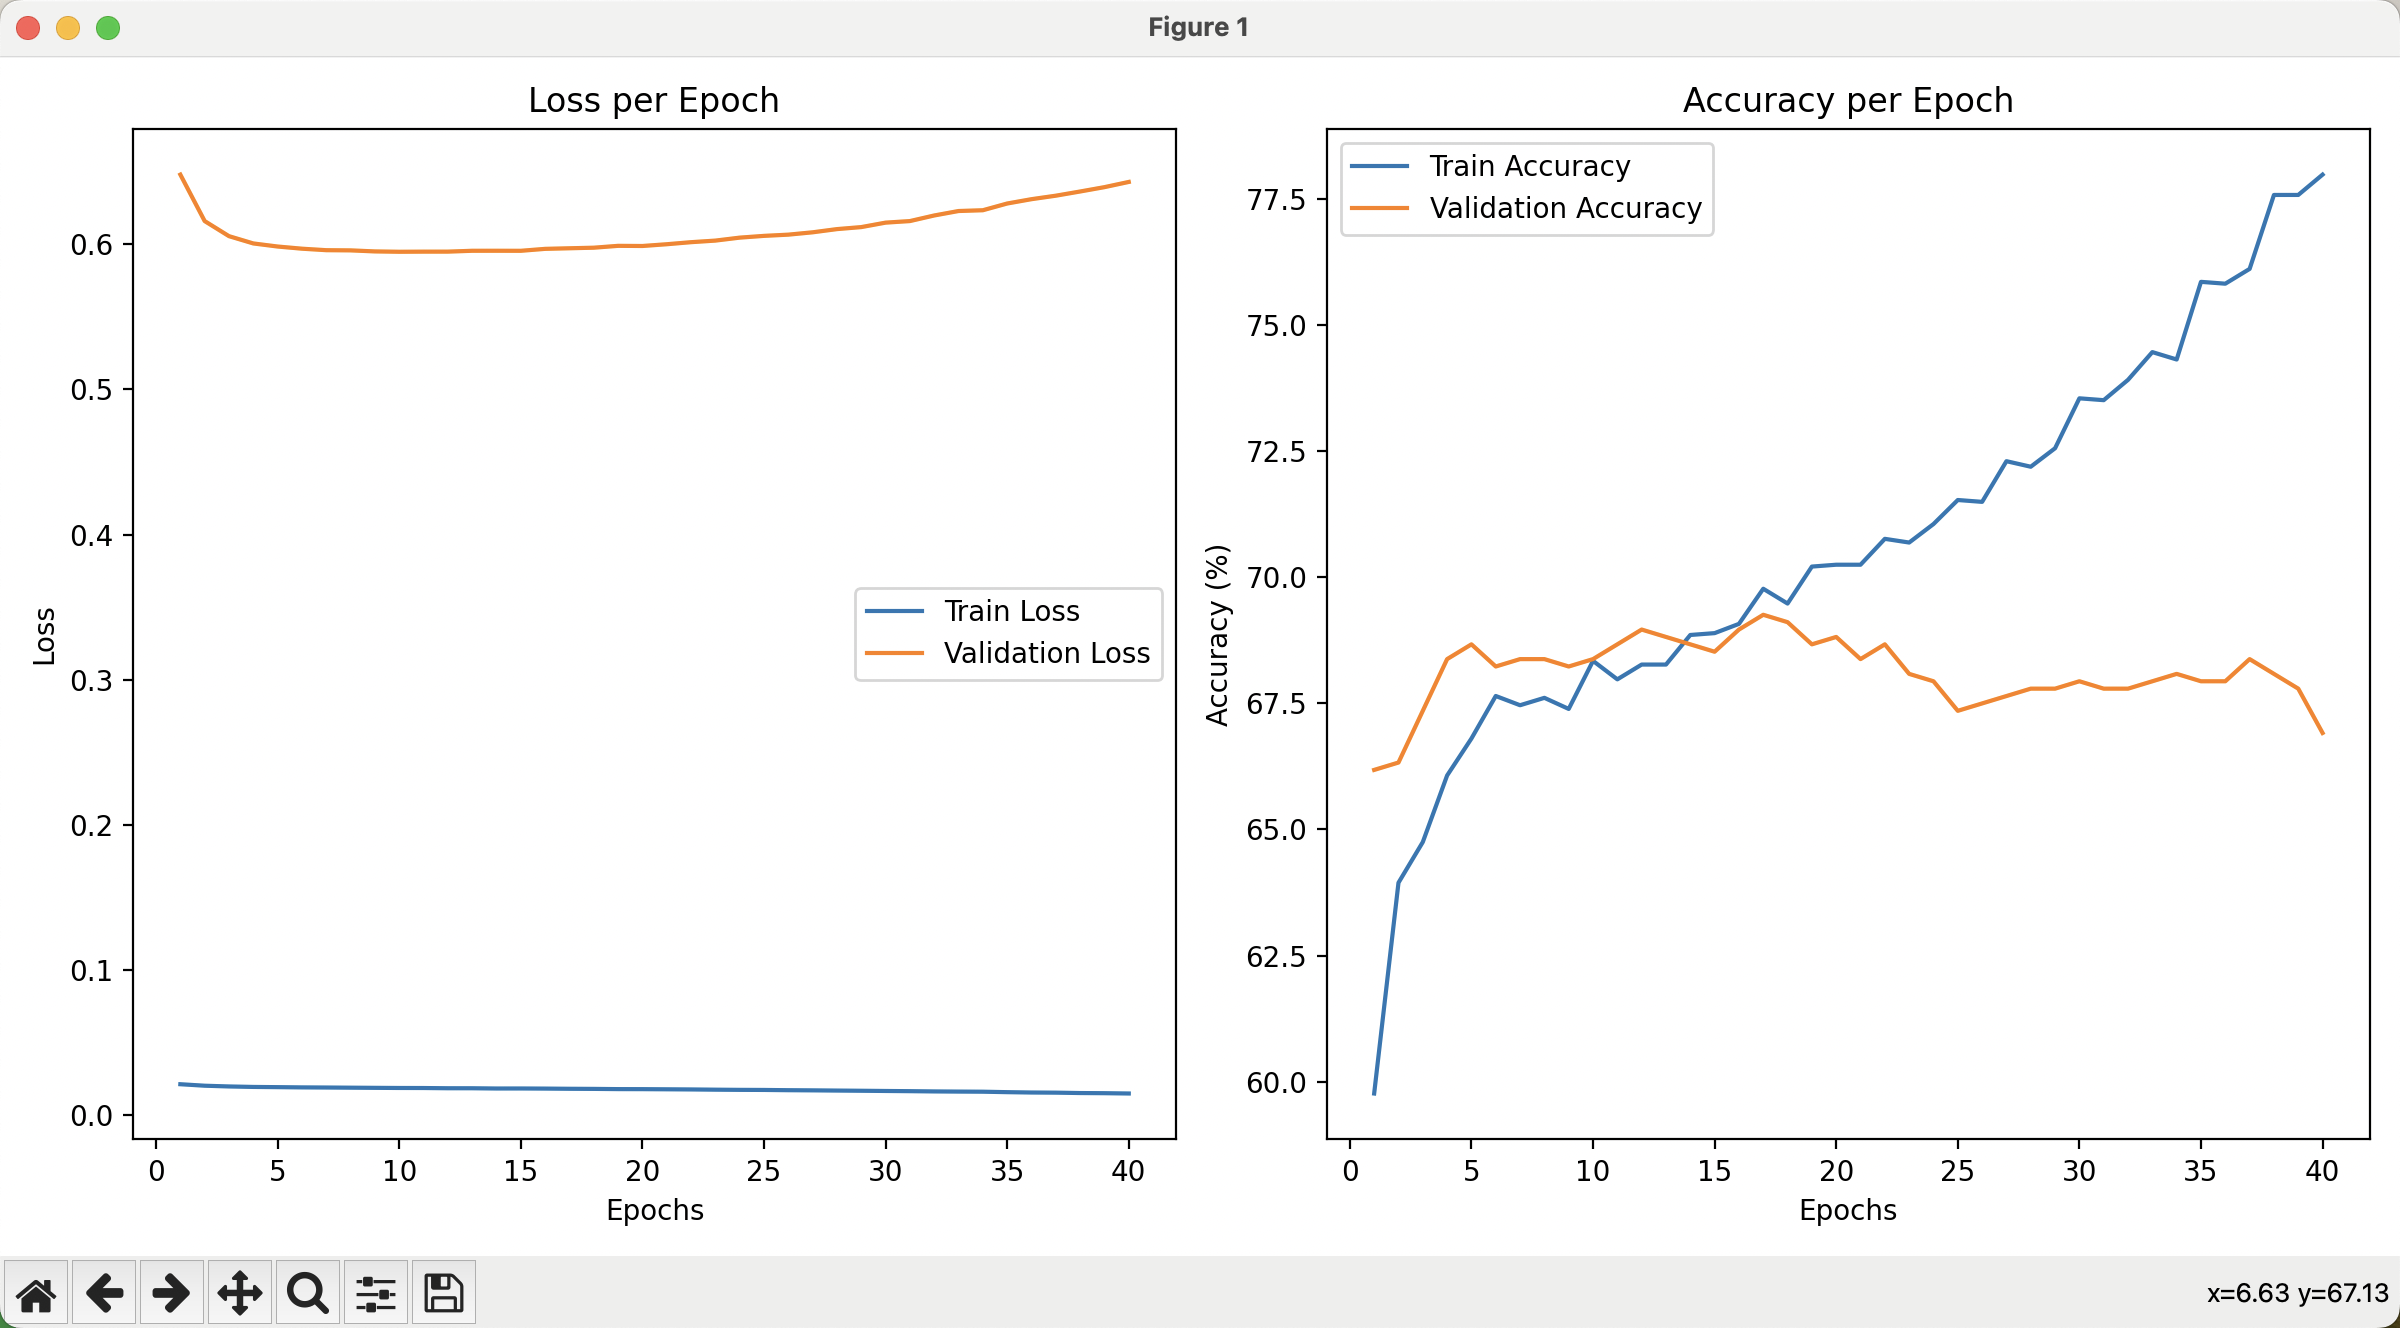
\includegraphics[height=0.55\linewidth]{Figures/3-40.png}
        \caption*{(a) 40 epoch}
    \end{minipage}
    % \hfill % 添加空白填充,确保图片之间有一些间隔
    \begin{minipage}{0.49\linewidth}
        \centering
        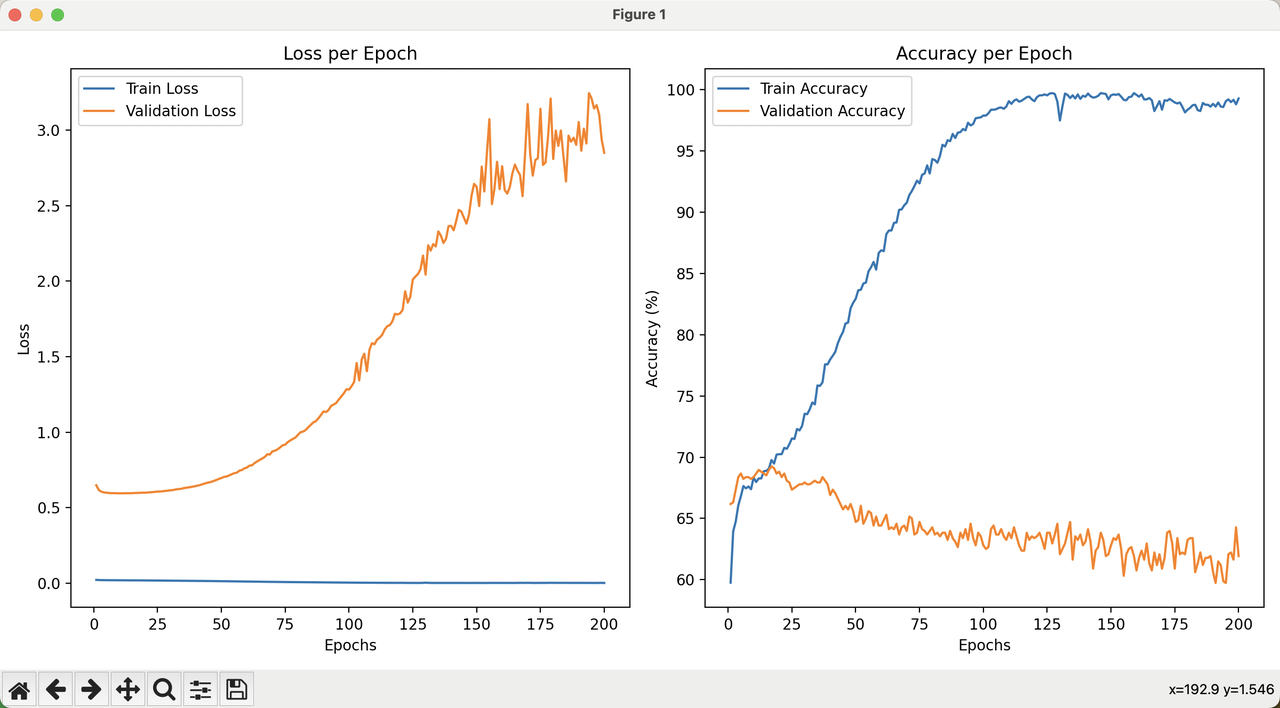
\includegraphics[height=0.55\linewidth]{Figures/3-200.png}
        \caption*{(b) 200 epoch}
    \end{minipage}
    \caption{RNA\_Regression\_3模型结果比较}
    \label{fig:RNA-Regression-3 Compare}
\end{figure}

从三个模型的拟合效果看,training loss都能很快地降低到0,validation loss在下降时则受到了一定的限制,无法充分与0靠近。这说明在RNA中可能还蕴含其他生物信息学的信息,仅仅使用K-mer或者Transformer的编码方式,还没能够充分找寻到其中的信息。比较图\ref{fig:RNA-Regression Compare}和图\ref{fig:RNA-Regression-2 Compare},添加了批归一化层的模型2在的training accuracy在不断的训练中展示出一定的波动性,抑制了模型的快速过拟合,使得training accuracy不断增加的同时,validation accuracy也能保持在高位。相比之下,没有添加批归一化层的模型1在训练轮次较高时出现了validation accuracy的下降,过拟合问题较为严重。同时,从表\ref{tab:CNN方法网络架构比较}的第1、2和4、5行也可以看出,随着轮次的增加,模型2最终的test accuracy仍能够继续上升,而模型1则没有显著的增长。

相比之下,模型3虽然结构更复杂,但是过拟合收敛的速度也大大增加。随着训练轮次的增加,validation accuracy先降低,而后大幅增加。training accuracy虽然能够迅速逼近100\%,但是最终的test accuracy则逐步走低,不如模型1和模型2。因此,综合比较下来,\textbf{我们选择RNA\_Regression\_2模型作为主要使用的神经网络,其虽然结构简单,但足以完成任务要求,而且具有较高的鲁棒性}。


\subsection{隐层规模比较}

接下来,我们测试比较隐层中多少神经元数量比较适合我们当前的数据集规模和任务需求,其他参数选定为K-mer为2,模型RNA\_Regression\_2,训练epoch为200,结果如表\ref{tab:CNN方法隐层数量比较}所示。

\begin{table*}[h]
\centering
\footnotesize
\setlength{\tabcolsep}{5pt}
\caption{NN方法隐层数量比较}
\label{tab:CNN方法隐层数量比较}
{
    \begin{tabular}{ccccc}
    \toprule
    \textbf{hidden size} & \textbf{Train\_Loss}($\downarrow$) & \textbf{Val\_Loss}($\downarrow$)  & \textbf{Val\_Accuracy\%}($\uparrow$)  & \textbf{Test\_accuracy\%}($\uparrow$)
    \\
    \midrule
    100 & 0.0183 & 0.5947 & 68.23 & 70.00\\
    200 & 0.0180 & 0.5981 & 68.53 & 69.74\\
    300 & 0.0178 & 0.6005 & 68.08 & 69.21\\
    500 & 0.0174 & 0.6017 & 67.79 & 70.79\\
    700 & 0.0171 & 0.6027 & 67.35 & 69.47\\
    1000 & 0.0167 & 0.6060 & 67.79 & 69.47\\
    1500 & 0.0161 & 0.6089 & 66.62 & 70.26\\
    3000 & 0.0145 & 0.6149 & 68.08 & 67.63\\

    \bottomrule
    \end{tabular}
}
\end{table*}

从表\ref{tab:CNN方法隐层数量比较}中可以发现,当模型越来越复杂,也即是隐层数量越来越多时,模型对训练集的拟合效果越来越好,training loss逐渐降低,但与此同时validation loss逐渐升高,对检验集的泛化性效果逐渐变差,val accuracy先升高后降低。在后续的参数组合中,我们通过大量实验和测试,\textbf{得出隐层数量为330左右对我们的任务最为合适}。


\subsection{K-mer规模选择}
在确定了前面两个参数的基础上,我们探索使用什么样的K-mer编码效果最好。使用模型RNA\_Regression\_2,隐层数量330,训练轮次为200,分别取k为1,2,3,4,5来进行实验,结果如表\ref{tab:CNN方法K-mer编码比较}所示,训练过程中的loss和accuracy变化曲线如图\ref{fig:K-mer方法选择比较}所示。

\begin{table*}[h]
\centering
\footnotesize
\setlength{\tabcolsep}{5pt}
\caption{NN方法K-mer编码比较}
\label{tab:CNN方法K-mer编码比较}
{
    \begin{tabular}{cccccc}
    \toprule
    \textbf{K-mer} & \textbf{Train\_Loss}($\downarrow$) & \textbf{Val\_Loss}($\downarrow$)  & \textbf{Train\_Accuracy\%}($\uparrow$)  & \textbf{Val\_accuracy\%}($\uparrow$)  & \textbf{Test\_Accuracy\%}($\uparrow$)
    \\
    \midrule
    1 & 0.0208 & 0.6671 & 60.21 & 59.44 & 63.68\\
    2 & 0.0185 & 0.5936 & 69.22 & 68.81 & 71.05\\
    3 & 0.0096 & 0.7229 & 89.74 & 66.47 & 68.42\\
    4 & 0.0000 & 2.3061 & 100.00 & 63.69 & 63.16\\
    5 & 0.0000 & 4.9587 & 100.00 & 61.49 & 61.58\\
    \bottomrule
    \end{tabular}
}
\end{table*}

\begin{figure}[h]
    \centering
    \begin{minipage}{0.49\linewidth}
        \centering
        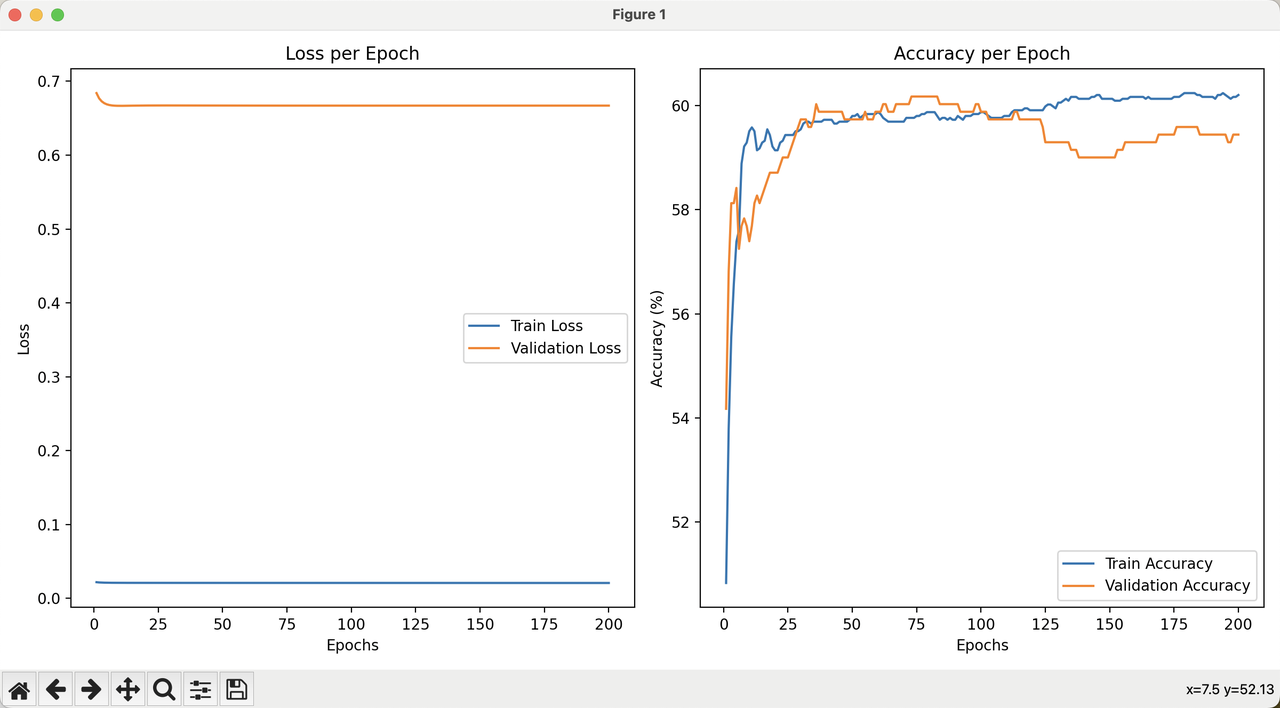
\includegraphics[height=0.55\linewidth]{Figures/k 1.png}
        \caption*{(a) 1-Mer}
    \end{minipage}
    % \hfill % 添加空白填充,确保图片之间有一些间隔
    \begin{minipage}{0.49\linewidth}
        \centering
        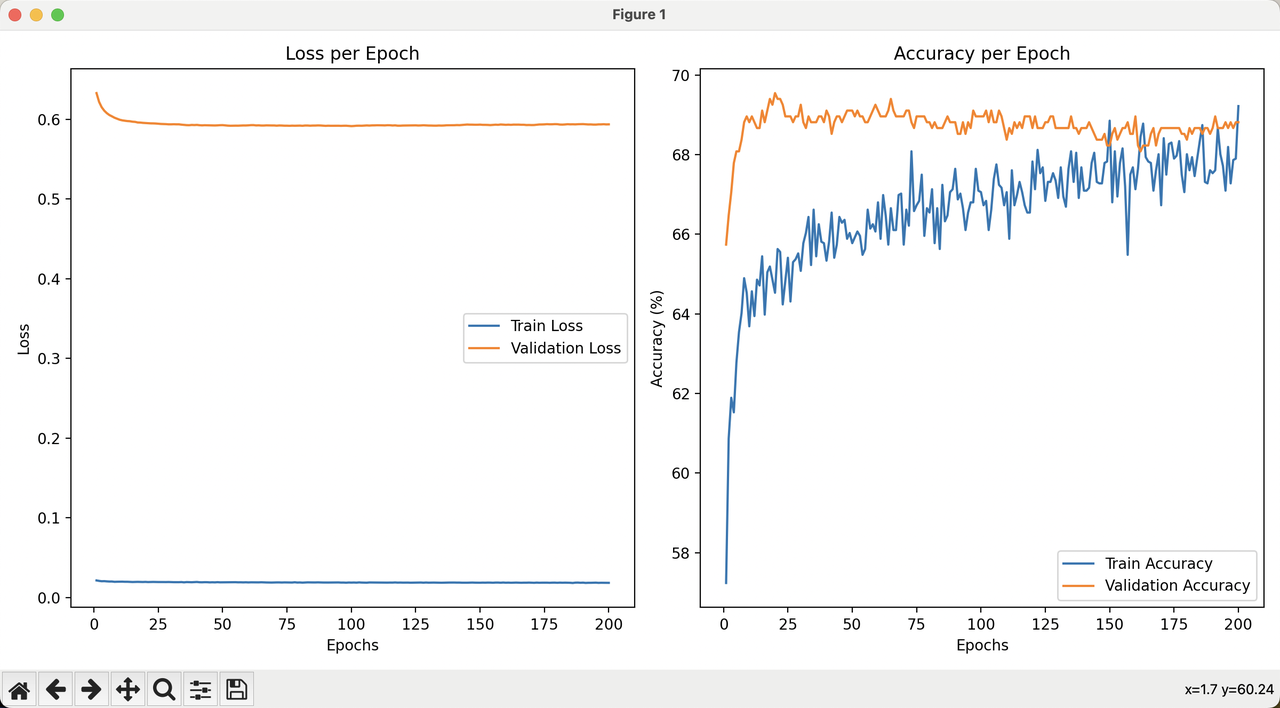
\includegraphics[height=0.55\linewidth]{Figures/k 2.png}
        \caption*{(b) 2-Mer}
    \end{minipage}
    \begin{minipage}{0.49\linewidth}
        \centering
        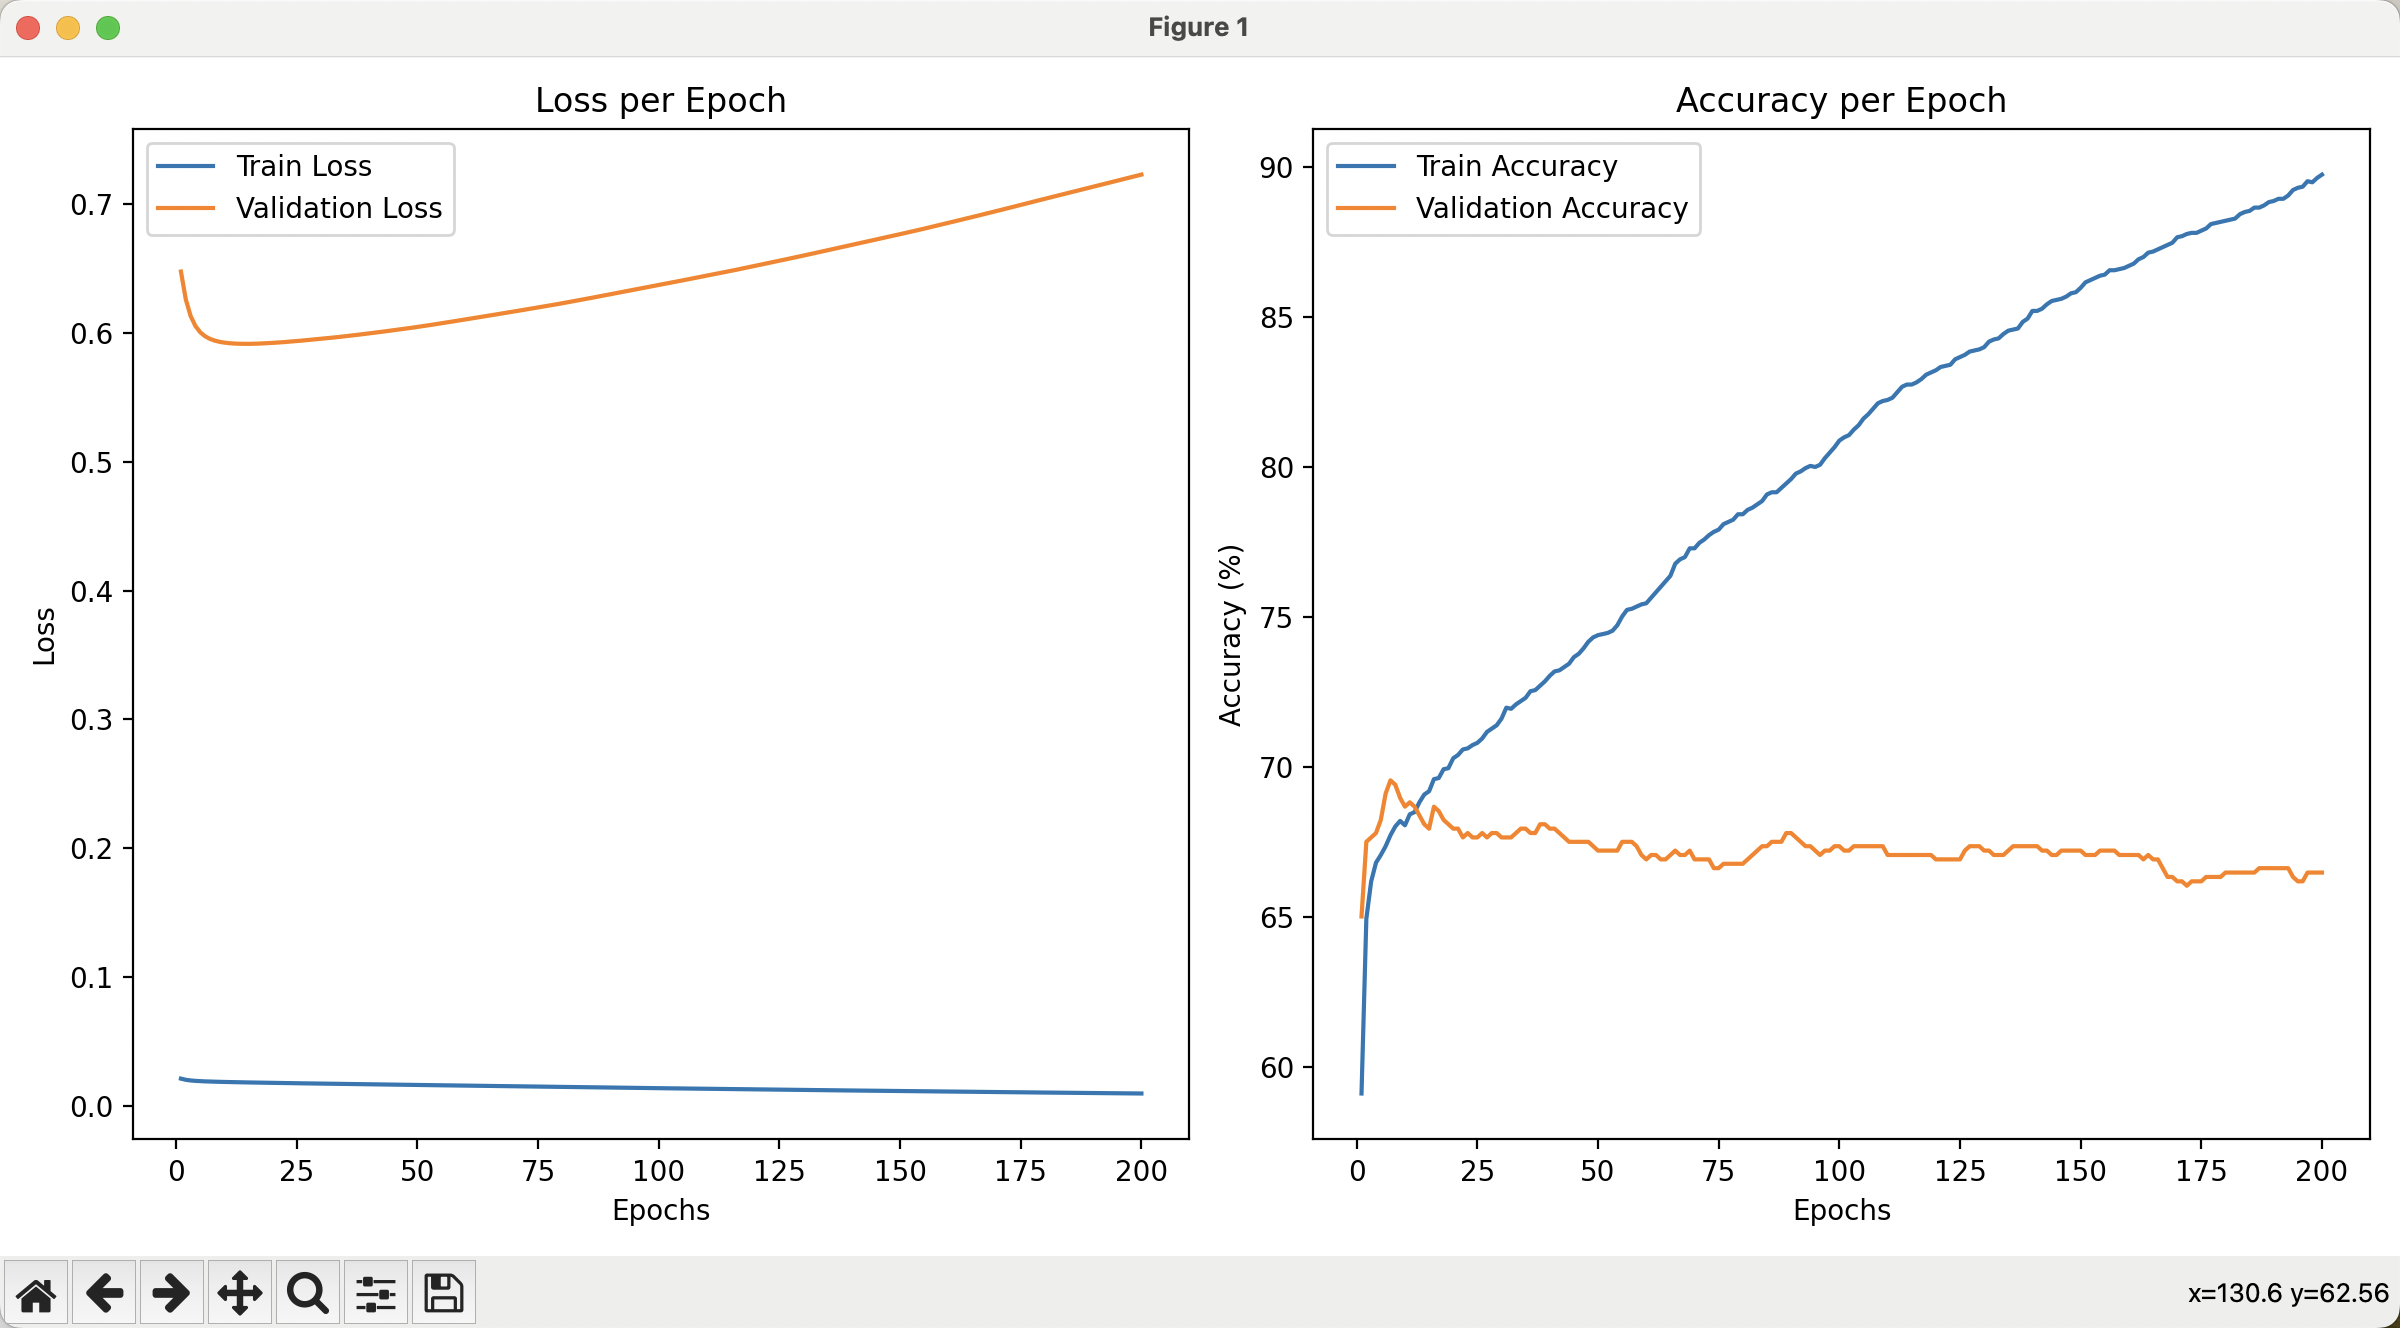
\includegraphics[height=0.55\linewidth]{Figures/k 3.png}
        \caption*{(a) 3-Mer}
    \end{minipage}
    % \hfill % 添加空白填充,确保图片之间有一些间隔
    \begin{minipage}{0.49\linewidth}
        \centering
        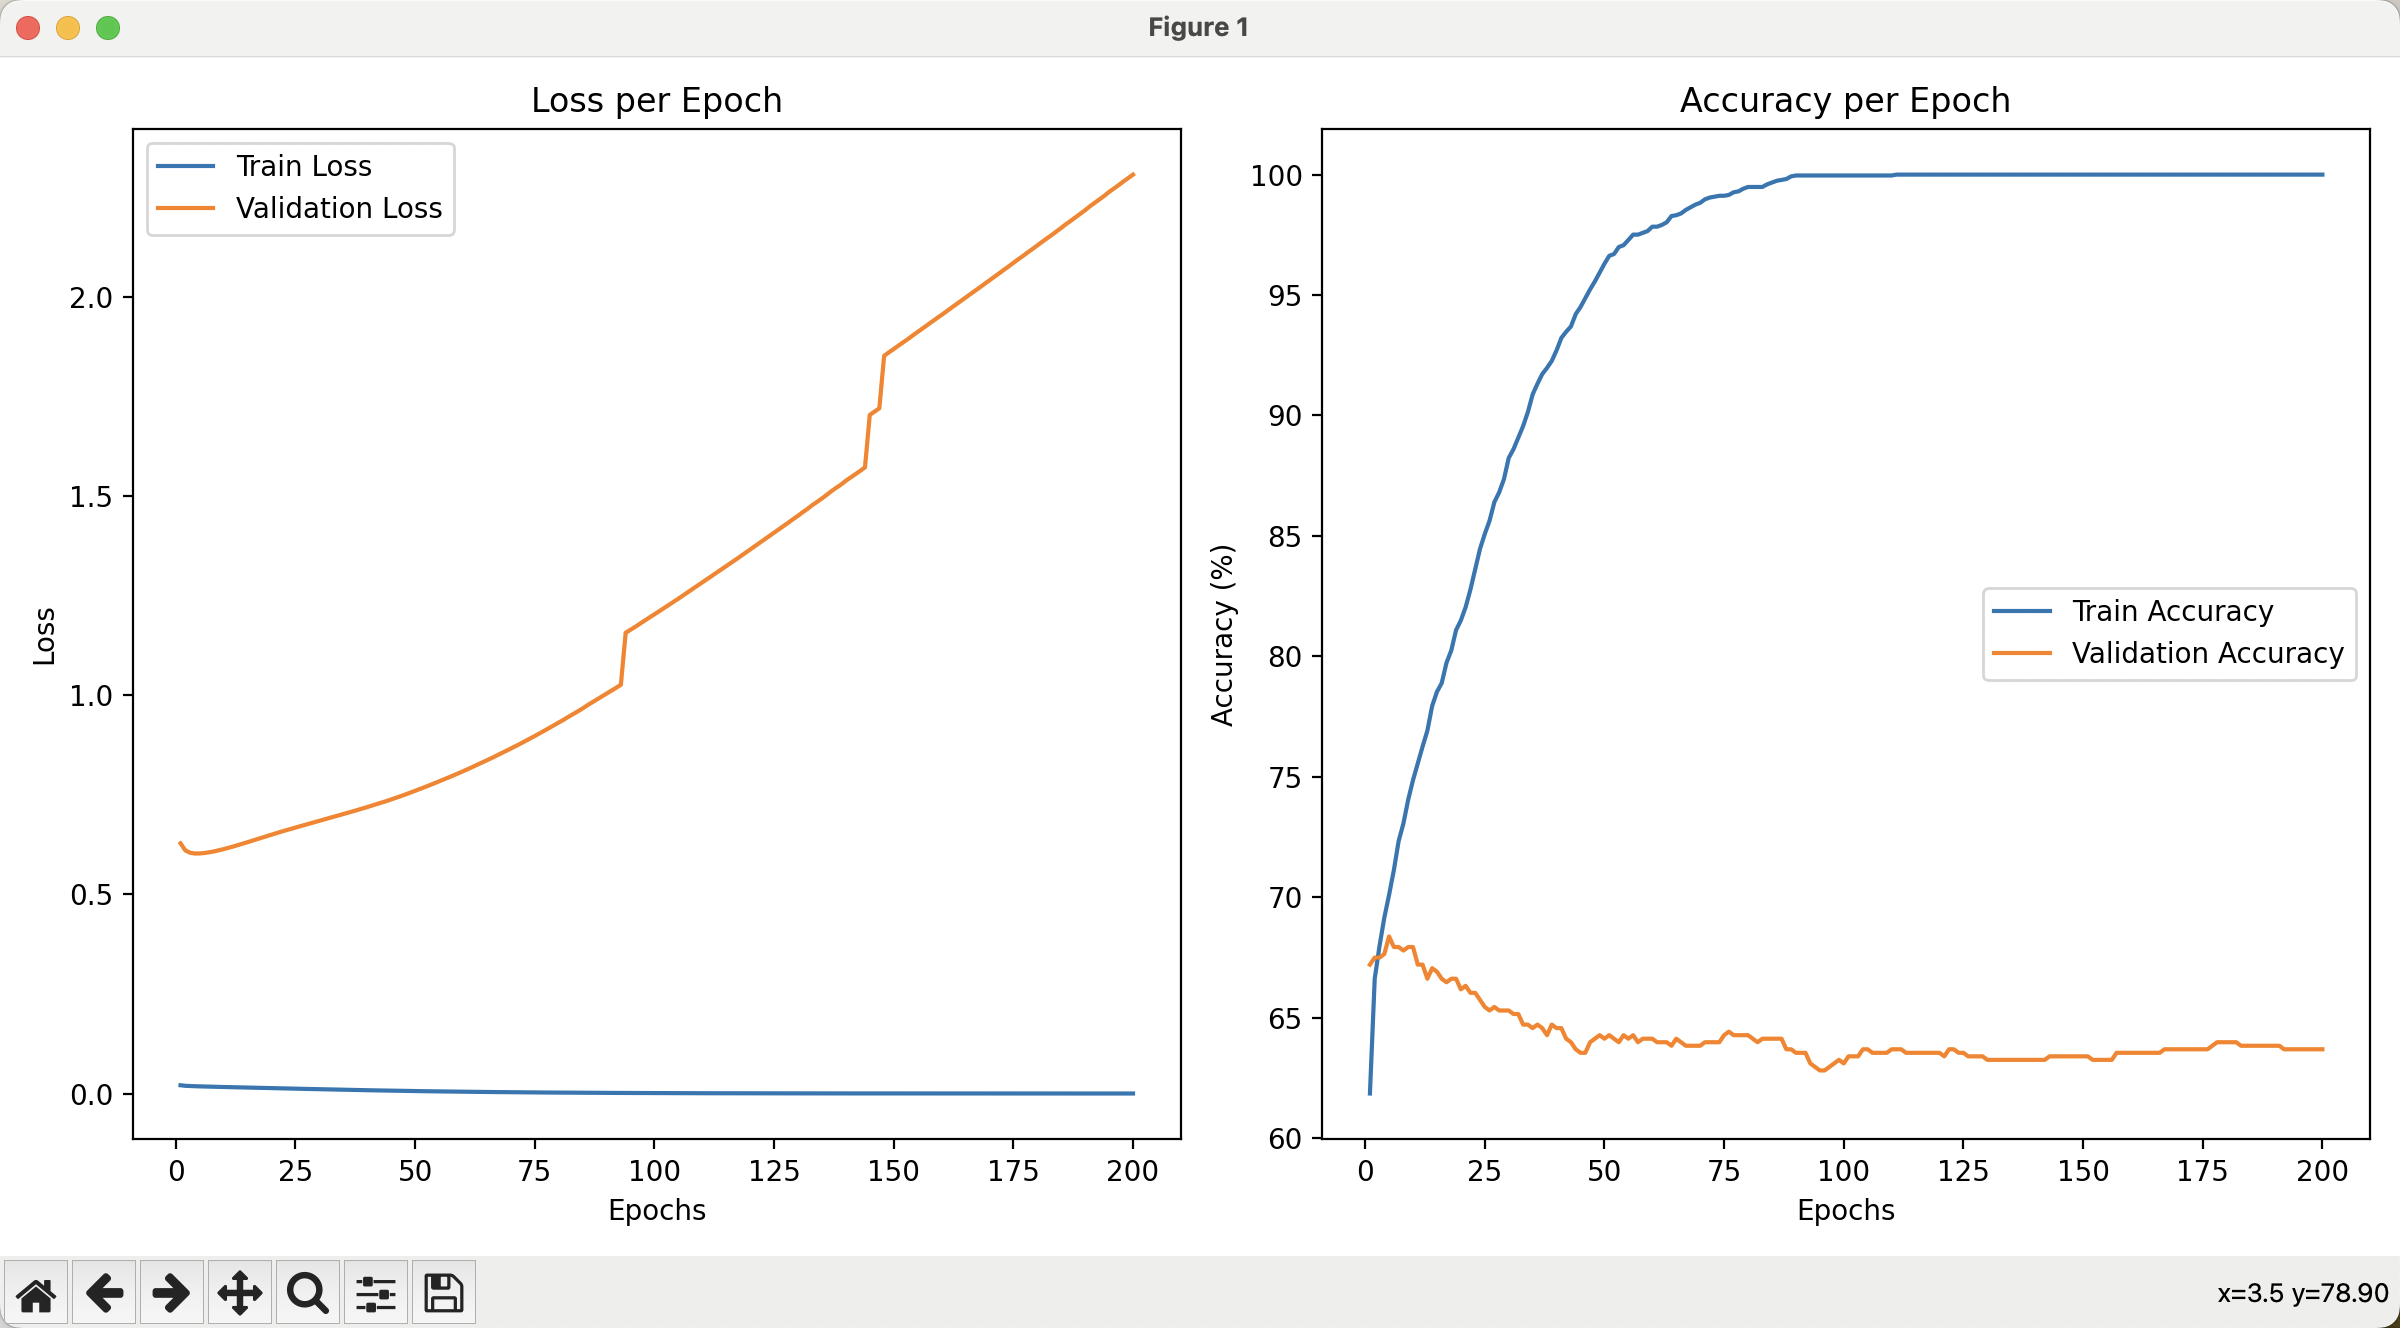
\includegraphics[height=0.55\linewidth]{Figures/k 4.png}
        \caption*{(b) 4-Mer}
    \end{minipage}
    \begin{minipage}{0.49\linewidth}
        \centering
        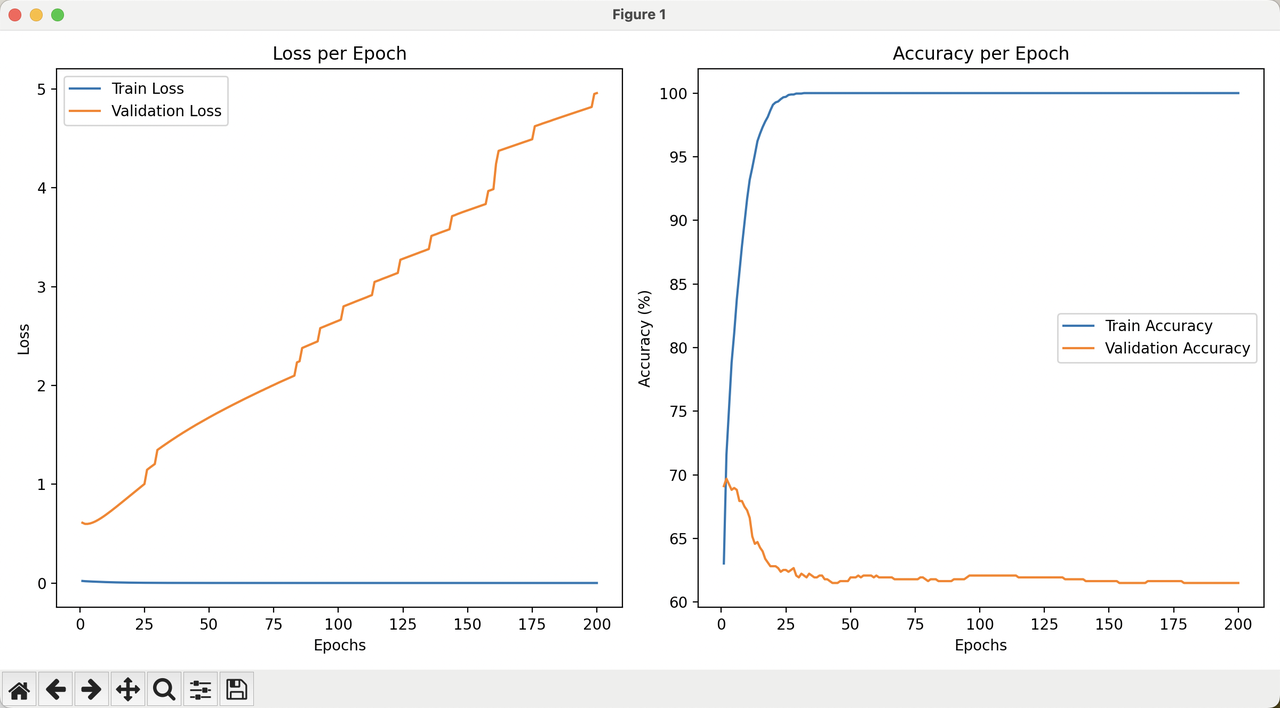
\includegraphics[height=0.55\linewidth]{Figures/k 5.png}
        \caption*{(b) 5-Mer}
    \end{minipage}
    \caption{K-mer方法选择比较}
    \label{fig:K-mer方法选择比较}
\end{figure}


从表中我们可以看出随着K的增加,test accuracy先增加后降低,在K=2的时候达到最佳效果。随着K的上升,说明编码的时候提取了更多训练集基因的独特信息,使得对training set拟合的收敛速度逐渐上升,比如使用5—Mer编码的水后,只需要20个epoch就可以近乎达到traing accuracy 100\%,但与此带来的是严重的泛化性问题,对4-Mer,5-Mer方法,validation loss在一开始非常短暂的下降之后开始急剧上升,validation loss与training loss背道而驰,这与我们的预期相反。

\textbf{最终,经过比较和测试,我们选择使用2—Mer编码方法来构建向量,表示RNA序列。}


\subsection{综合结果比较}
在前面的实验中,我们基于本数据集的RNA分类任务在争取更好的泛化性上有一定困难,当模型变得更加复杂的时候,泛化性效果反而降低。\textbf{经过多轮尝试比较,我们选定使用模型RNA\_Regression\_2,隐层规模330,2-Mer编码方式,最终的Validation Accuracy可达到68.81\%左右,接近70\%。对具体的训练轮数,我们选择validation loss下降到最低点的位置,作为最佳epoch数量,当epoch取2的时候,我们在测试集上达到的最佳准确度73.95\%。}下面,我们考虑使用课程中涉及的其他方法来进一步尝试是否有可能对预测分类效果做出进一步改善。


\section{支持向量机 Support Vector Machine}

\subsection{SVM的基本原理}


支持向量机(Support Vector Machine, SVM)是一种监督学习模型,广泛应用于分类和回归任务。SVM 的核心思想是寻找一个最优的超平面(hyperplane),将不同类别的数据点分开,并使得该超平面与各类别最近的数据点(称为支持向量)的距离最大化。

考虑一个线性可分的二分类问题,假设数据集为 $\{(\mathbf{x}_i, y_i)\}_{i=1}^N$,其中 $\mathbf{x}_i \in \mathbb{R}^d$ 表示第 $i$ 个样本的特征向量,$y_i \in \{-1, +1\}$ 表示其类别标签。SVM 旨在找到一个超平面 $ \mathbf{w}^\top \mathbf{x} + b = 0 $ 来分隔这两类数据。其中,边界间隔(margin)是指超平面到最近支持向量的距离。最大化边界间隔有助于提高分类器的泛化能力,SVM 的优化问题可以表述为:

\begin{equation}
\begin{aligned}
& \underset{\mathbf{w}, b}{\text{min}} && \frac{1}{2} \|\mathbf{w}\|^2 \\
& \text{s.t.} && y_i (\mathbf{w}^\top \mathbf{x}_i + b) \geq 1, \quad \forall i = 1, 2, \dots, N
\end{aligned}
\end{equation}

\begin{itemize}
    \item \textbf{目标函数} $\frac{1}{2} \|\mathbf{w}\|^2$:最小化权重向量的范数,从而最大化间隔。
    \item \textbf{约束条件} $y_i (\mathbf{w}^\top \mathbf{x}_i + b) \geq 1$:确保所有样本被正确分类,并且支持向量满足等式 $y_i (\mathbf{w}^\top \mathbf{x}_i + b) = 1$。
\end{itemize}

为了求解上述优化问题,引入拉格朗日乘子 $\alpha_i$,形成拉格朗日函数:

\begin{equation}
L(\mathbf{w}, b, \alpha) = \frac{1}{2} \|\mathbf{w}\|^2 - \sum_{i=1}^N \alpha_i \left[ y_i (\mathbf{w}^\top \mathbf{x}_i + b) - 1 \right]
\end{equation}

通过对偶性,可以将其转化为对偶问题:

\begin{equation}
\begin{aligned}
& \underset{\alpha}{\text{max}} && \sum_{i=1}^N \alpha_i - \frac{1}{2} \sum_{i,j=1}^N \alpha_i \alpha_j y_i y_j \mathbf{x}_i^\top \mathbf{x}_j \\
& \text{s.t.} && \alpha_i \geq 0, \quad \forall i \\
& && \sum_{i=1}^N \alpha_i y_i = 0
\end{aligned}
\end{equation}

通过求解对偶问题,可以得到优化的拉格朗日乘子 $\alpha_i$,从而求解出最优的 $\mathbf{w}$ 和 $b$。

但是,在实际应用中,数据往往不可完全线性分割,或者存在噪声和离群点。为了处理这类情况,引入软间隔(soft margin)概念,允许部分样本违背间隔约束,故引入松弛变量 $\xi_i \geq 0$,优化问题变为:

\begin{equation}
\begin{aligned}
& \underset{\mathbf{w}, b, \xi}{\text{min}} && \frac{1}{2} \|\mathbf{w}\|^2 + C \sum_{i=1}^N \xi_i \\
& \text{s.t.} && y_i (\mathbf{w}^\top \mathbf{x}_i + b) \geq 1 - \xi_i, \quad \forall i \\
& && \xi_i \geq 0, \quad \forall i
\end{aligned}
\end{equation}

\begin{itemize}
    \item \textbf{目标函数}:在最大化边界间隔的同时,最小化违约(通过 $\xi_i$ 表示)。
    \item \textbf{参数 $C$}:控制间隔最大化和误分类样本之间的权衡。较大的 $C$ 强调正确分类,较小的 $C$ 强调间隔宽度。
\end{itemize}

\subsection{SVM中的核方法(Kernel Method)}

当数据在原始空间中不可线性分割时,核方法通过将数据映射到高维特征空间,使其在高维空间中线性可分。核方法的核心思想是通过核函数计算数据在高维空间中的内积,而无需显式进行高维映射。

核函数 $K(\mathbf{x}_i, \mathbf{x}_j)$ 定义为:

\begin{equation}
K(\mathbf{x}_i, \mathbf{x}_j) = \phi(\mathbf{x}_i)^\top \phi(\mathbf{x}_j)
\end{equation}

其中 $\phi(\cdot)$ 是将数据映射到高维特征空间的映射函数。常用的核函数有:

\begin{enumerate}
    \item \textbf{线性核(Linear Kernel)}
    \begin{equation}
    K(\mathbf{x}_i, \mathbf{x}_j) = \mathbf{x}_i^\top \mathbf{x}_j
    \end{equation}
    \begin{itemize}
        \item \textbf{映射原理}:实际上不进行任何映射,直接在原始空间中操作。
        \item \textbf{特点}:适用于线性可分的数据,计算简单高效。
    \end{itemize}
    
    \item \textbf{多项式核(Polynomial Kernel)}
    \begin{equation}
    K(\mathbf{x}_i, \mathbf{x}_j) = (\gamma \mathbf{x}_i^\top \mathbf{x}_j + r)^d
    \end{equation}
    其中 $\gamma > 0$ 是核系数,$r$ 是常数项,$d$ 是多项式的度数。
    \begin{itemize}
        \item \textbf{映射原理}:将数据映射到一个包含所有特征交互项的高维空间,例如二次、多次特征。
        \item \textbf{特点}:通过调整参数 $d$、$\gamma$ 和 $r$,可以控制模型的复杂度和拟合能力。适用于具有多项式关系的数据。
    \end{itemize}
    
    \item \textbf{径向基函数核(Radial Basis Function Kernel, RBF Kernel)}
    \begin{equation}
    K(\mathbf{x}_i, \mathbf{x}_j) = \exp(-\gamma \|\mathbf{x}_i - \mathbf{x}_j\|^2)
    \end{equation}
    其中 $\gamma > 0$ 是核宽度参数。
    \begin{itemize}
        \item \textbf{映射原理}:将数据映射到\textbf{无限维}的特征空间,能够处理非常复杂的非线性关系。
        \item \textbf{特点}:具有局部性,能有效处理具有复杂边界的数据。参数 $\gamma$ 控制单个样本的影响范围,较大的 $\gamma$ 值会导致模型更加复杂,容易过拟合。
    \end{itemize}
    
    \item \textbf{Sigmoid核(Sigmoid Kernel)}
    \begin{equation}
    K(\mathbf{x}_i, \mathbf{x}_j) = \tanh(\gamma \mathbf{x}_i^\top \mathbf{x}_j + r)
    \end{equation}
    \begin{itemize}
        \item \textbf{映射原理}:类似于神经网络中的激活函数,通过双曲正切函数实现非线性映射。
        \item \textbf{特点}:具有神经网络的非线性特性。参数 $\gamma$ 和 $r$ 需要调优,以确保模型的收敛性和性能。在实际应用中较少使用,通常用于特定类型的数据和任务。
    \end{itemize}
\end{enumerate}

\subsection{模型框架搭建}
基于前面神经网络方法的架构和流程,我们对修改其方法为支持向量机,同时通过args传入参数的方法设置核方法使用的卷积核以及一系列其他参数。具体代码实现的流程仍然是读入编码序列,标准化处理数据,初始化SVM模型,进行训练,评估验证集测试集效果等等。具体函数实现如下:

\begin{lstlisting}
# 分类函数 - 使用 SVM
def classification_with_svm(training_file, test_file, k=3, kernel='rbf', C=1.0, gamma='scale'):
    train_data = pd.read_csv(training_file)
    test_data = pd.read_csv(test_file)

    X_train = [kmer_encoding(seq, k) for seq in train_data.iloc[:, 2]]  # 第3列为RNA序列
    y_train = train_data.iloc[:, 3].values  # 第4列为标签
    
    X_test = [kmer_encoding(seq, k) for seq in test_data.iloc[:, 2]]
    y_test = test_data.iloc[:, 3].values
    
    X_train = np.array(X_train)
    X_test = np.array(X_test)

    scaler = StandardScaler()
    X_train = scaler.fit_transform(X_train)
    X_test = scaler.transform(X_test)
    
    X_train, X_val, y_train, y_val = train_test_split(X_train, y_train, test_size=0.2, random_state=42, stratify=y_train)
    
    model = SVC(kernel=kernel, C=C, gamma=gamma, probability=True, random_state=42)

    model.fit(X_train, y_train)

    y_val_pred = model.predict(X_val)
    val_accuracy = accuracy_score(y_val, y_val_pred)
    print(f"Validation Accuracy: {val_accuracy * 100:.2f}%")
    
    y_test_pred = model.predict(X_test)
    test_accuracy = accuracy_score(y_test, y_test_pred)
    print(f"Test Accuracy: {test_accuracy * 100:.2f}%")

    print("\nClassification Report (Test Set):")
    print(classification_report(y_test, y_test_pred))
    
    return model
\end{lstlisting}


\subsection{分类效果分析}
在SVM方法中,我们也初步探索了K-Mer编码K的值,以及核函数的选择对于RNA分类任务能带来多少提升,并比较他们之间的差异,如表\ref{tab:SVM方法RNA分类}所示。


\begin{table*}[h]
\centering
\footnotesize
\setlength{\tabcolsep}{5pt}
\caption{SVM方法RNA分类结果}
\label{tab:SVM方法RNA分类}
{
    \begin{tabular}{ccccc}
    \toprule
    \textbf{No.} & \textbf{K-Mer} & \textbf{Kernel}  & \textbf{Validation\_Accuracy\%}($\uparrow$)  & \textbf{Test\_accuracy\%}($\uparrow$)
    \\
    \midrule
    1 & 1 & RBF & 59.88 & 62.11 \\
    2 & 2 & RBF & 68.37 & 70.00 \\
    3 & 3 & RBF & 69.40 & 70.00 \\
    4 & 4 & RBF & 68.67 & 70.00\\
    5 & 5 & RBF & 67.35 & 68.16\\
    6 & 3 & Linear & 68.52 & 69.21 \\
    7 & 3 & Polynomial & 65.74 & 67.89\\
    8 & 3 & Sigmoid & 59.15 & 57.37 \\
    \bottomrule
    \end{tabular}
}
\end{table*}

从表中可以看出,SVM方法下采用3-Mer编码得到的分类效果最好,能够平衡RNA序列足够的特征采集以及过拟合之间的关系。同时,对3-Mer编码的结果采用四种常用的Kernel进行SVM算法分类发现,RBF Kernel的效果最好。因为RBF将向量映射到了一个无限维的空间中,最大程度上保留了其特征,也能够处理非常复杂的非线性关系。相比之下,Sigmoid核通过双曲正切函数实现非线性映射,对于输入值较大和较小的部分,容易出现梯度消失,不利于训练和分类的进行,效果最差。

\textbf{最终,在支持向量机SVM方法的框架下,我们选择3—Mer编码,利用RBF Kernel作为核函数来描述两个输入样本之间的关系,映射到无限维空间中,最终分类测试准确度也能达到70\%,略微逊色于神经网络方法。同时,也难以实现分类准确度的突破增长,未体现出明显优势。}

\section{决策树集成学习 Ensemble Learning}

\subsection{AdaBoost算法}
AdaBoost(Adaptive Boosting,自适应提升)是一种集成学习方法,旨在通过组合多个弱分类器(通常是简单的模型,如决策树)来构建一个强分类器。AdaBoost通过迭代地训练弱分类器,并在每一轮中调整样本权重,使得后续的分类器更关注之前分类错误的样本,从而提高整体分类性能。算法其过程包括以下几个步骤:

\begin{enumerate}
    \item \textbf{初始化样本权重}:为每个训练样本分配相等的初始权重。
    \item \textbf{迭代训练弱分类器}:
    \begin{itemize}
        \item 在每一轮迭代中,训练一个弱分类器,基于当前样本权重。
        \item 计算弱分类器的错误率。
        \item 计算该分类器的权重,反映其在最终模型中的重要性。
        \item 更新样本权重,使得被错误分类的样本在下一轮中权重增加,正确分类的样本权重减少。
    \end{itemize}
    \item \textbf{组合弱分类器}:通过加权投票或加权求和的方式,将所有弱分类器的输出结合起来,形成最终的强分类器。
\end{enumerate}

\textbf{首先,是初始化过程。}对于训练集中的每个样本 \( i \),初始化权重 \( w_i^{(1)} \) 为相等:

\begin{equation}
w_i^{(1)} = \frac{1}{N}, \quad \forall i = 1, 2, \dots, N
\end{equation}

其中,\( N \) 是训练样本的总数。

\textbf{第二步,迭代过程。}AdaBoost在每一轮 \( t = 1, 2, \dots, T \) 中执行以下步骤:

\begin{enumerate}
    \item \textbf{训练弱分类器}:
    
    使用当前权重分布 \( \{w_i^{(t)}\} \) 训练一个弱分类器 \( h_t \)。
    
    \item \textbf{计算分类错误率}:
    
    弱分类器 \( h_t \) 的加权错误率 \( \epsilon_t \) 定义为:
    
    \begin{equation}
    \epsilon_t = \frac{\sum_{i=1}^N w_i^{(t)} \mathbb{I}(y_i \neq h_t(x_i))}{\sum_{i=1}^N w_i^{(t)}}
    \end{equation}
    
    其中,\( \mathbb{I}(\cdot) \) 是指示函数,当括号内条件为真时取1,否则取0。
    
    \item \textbf{计算分类器权重}:
    
    弱分类器 \( h_t \) 的权重 \( \alpha_t \) 根据其错误率计算:
    
    \begin{equation}
    \alpha_t = \frac{1}{2} \ln \left( \frac{1 - \epsilon_t}{\epsilon_t} \right)
    \end{equation}
    
    该权重反映了分类器的可信度,错误率越低,权重越高。
    
    \item \textbf{更新样本权重}:
    
    更新样本权重以强调被错误分类的样本:
    
    \begin{equation}
    w_i^{(t+1)} = w_i^{(t)} \exp \left( -\alpha_t y_i h_t(x_i) \right)
    \end{equation}
    
    然后进行归一化处理,使得权重之和为1:
    
    \begin{equation}
    w_i^{(t+1)} = \frac{w_i^{(t+1)}}{\sum_{j=1}^N w_j^{(t+1)}}
    \end{equation}
\end{enumerate}

\textbf{第三步,得到最终分类器。}

经过 \( T \) 轮迭代后,最终的强分类器 \( H(x) \) 通过加权多数投票或加权求和的方式得到:

\begin{equation}
H(x) = \text{sign} \left( \sum_{t=1}^T \alpha_t h_t(x) \right)
\end{equation}


\subsection{AdaBoost效果分析}

在AdaBoost方法中,我们对超参数的选择做出了一些调整和尝试,包括分类层深度depth,弱学习器数量,K-mer,学习率learning rate等等,并对validation accuracy和test accuracy进行比较测试,结果如表\ref{tab:AdaBoost算法效果比较}所示:

\begin{table*}[h]
\centering
\footnotesize
\setlength{\tabcolsep}{5pt}
\caption{AdaBoost算法效果比较}
\label{tab:AdaBoost算法效果比较}
{
    \begin{tabular}{ccccccc}
    \toprule
    \textbf{No.} & \textbf{depth} & \textbf{弱学习器数量} & \textbf{K-mer} & \textbf{learning rate}  & \textbf{Validation\_Accuracy\%}($\uparrow$)  & \textbf{Test\_accuracy\%}($\uparrow$)
    \\
    \midrule
    1 & 1 & 500 & 2 & 0.1 & 67.64 & 71.05 \\
    2 & 1 & 500 & 2 & 0.05 & 67.20 & 72.37 \\
    3 & 1 & 500 & 3 & 0.05 & 65.45 & 66.32 \\
    4 & 1 & 250 & 3 & 0.05 & 65.59 & 69.74 \\
    5 & 1 & 125 & 3 & 0.05 & 66.76 & 70.26 \\
    6 & 1 & 100 & 3 & 0.05 & 67.64 & 69.47 \\
    7 & 1 & 80 & 3 & 0.05 & 66.62 & 68.68 \\
    8 & 2 & 200 & 2 & 0.05 & 66.76 & 72.37 \\
    9 & 3 & 100 & 2 & 0.05 & 66.18 & 72.37 \\
    \bottomrule
    \end{tabular}
}
\end{table*}

\textbf{首先,我们在深度只有1的弱学习器中进行分析。}从第1、2组实验,我们发现更大的学习率会使模型更快收敛,但和前面的尝试类似,会带来更为严重的过拟合和泛化性误差问题。经过进一步的比较和尝试,我们选择0.05作为我们主要的学习率取值。

通过第3、4、5、6、7组实验,我们发现对3-Mer编码方法,100至200个弱学习器较为合适;而与第2组实验比较,对2-Mer编码方法,500个左右弱学习器效果较好。与前面的尝试结果类似,K与需要的弱学习器的数量负相关,同时,采用3-Mer编码仍然会带来较为严重的过拟合问题,相比2-Mer编码方法,其准确度产生一定程度的下降。

\textbf{其次,我们探索深度对学习效果的影响。}以实验2为基准,分别使用深度为2和3的弱学习器进行训练,经过尝试发现其最终测试效果差距不大,但是在训练过程中的验证集上其validation accuracy随着深度的增加略有下降。同时,达到相同的测试准确度,深度越深,弱学习器所需的数量越少,训练收敛的速度越快。

\textbf{最终,在AdaBoost方法中,我们选择500个深度为1的弱学习器,学习率0.05,使用2-Mer编码进行集成学习训练,最终在验证集上准确率达到67.20\%,在测试集上准确率达到72.37\%,与运用神经网络方法的结果相近。}

\subsection{自动参数筛选设计}
在对模型超参数进行调整优化的过程中,我们设计了自动参数测试筛选流程。我们以n\_estimators为例,传入一系列候选的参数,或者一定范围内,给定步长的参数等等,通过cross validation方法,自动对这些参数进行测试验证,最终选取效果最好的最终选用。同时,也留出了进一步扩展的空间,对超参数组进行训练调试。具体代码实现如下:

\begin{lstlisting}
def select_n_estimators(training_file, test_file, k, n_estimators_range, cv=5, scoring='accuracy', learning_rate=0.1, max_depth=3):
    train_data = pd.read_csv(training_file)
    test_data = pd.read_csv(test_file)

    X_train = [kmer_encoding(seq, k) for seq in train_data.iloc[:, 2]]  # 第3列为RNA序列
    y_train = train_data.iloc[:, 3].values  # 第4列为标签
    
    X_test = [kmer_encoding(seq, k) for seq in test_data.iloc[:, 2]]
    y_test = test_data.iloc[:, 3].values

    X_train = np.array(X_train)
    X_test = np.array(X_test)

    scaler = StandardScaler()
    X_train = scaler.fit_transform(X_train)
    X_test = scaler.transform(X_test)

    X_train, X_val, y_train, y_val = train_test_split(X_train, y_train, test_size=0.2, random_state=42, stratify=y_train)
    
    results = {}
    for n_estimators in n_estimators_range:
        print(f"Evaluating n_estimators={n_estimators}...")
        model = XGBClassifier(
            n_estimators=n_estimators,
            learning_rate=learning_rate,
            max_depth=max_depth,
            use_label_encoder=False,
            eval_metric='logloss',
            random_state=42
        )
        scores = cross_val_score(model, X_train, y_train, cv=cv, scoring=scoring)
        results[n_estimators] = np.mean(scores)
        print(f"Mean CV Accuracy for n_estimators={n_estimators}: {results[n_estimators]:.4f}")

    best_n_estimators = max(results, key=results.get)
    print(f"\nBest n_estimators: {best_n_estimators} with Mean CV Accuracy: {results[best_n_estimators]:.4f}")
    return best_n_estimators, results

\end{lstlisting}


\subsection{XGBoost算法}

XGBoost(eXtreme Gradient Boosting)是一种高效的梯度提升框架,其核心算法基于梯度提升决策树(Gradient Boosting Decision Trees, GBDT)。与AdaBoost相比,XGBoost在多个方面进行了显著的改进和优化,从而提升了模型的性能和计算效率。

XGBoost的基本思想是通过逐步构建和组合多个决策树来优化目标函数。具体来说,XGBoost通过最小化一个包含损失函数和正则化项的目标函数来训练模型。目标函数可以表示为:

\begin{equation}
\mathcal{L}(\phi) = \sum_{i=1}^n l(y_i, \hat{y}_i) + \sum_{k=1}^K \Omega(f_k),
\end{equation}

其中,$l$ 是损失函数,用于衡量预测值 $\hat{y}_i$ 与真实值 $y_i$ 之间的差异,$\Omega$ 是正则化项,用于控制模型的复杂度,$f_k$ 表示第 $k$ 棵决策树,$K$ 是树的总数。

与AdaBoost主要通过调整样本权重来关注难以分类的样本不同,XGBoost采用梯度下降的方法,通过优化目标函数的梯度方向来系统性地提升模型的整体性能。在每一轮迭代中,XGBoost构建一棵新的决策树来拟合当前模型的残差(即目标函数对预测值的梯度),其更新过程可以表示为:

\begin{equation}
\hat{y}^{(t)} = \hat{y}^{(t-1)} + \eta f_t(x),
\end{equation}

其中,$\eta$ 是学习率,$f_t(x)$ 是第 $t$ 棵新增的决策树。

为了防止过拟合,XGBoost在目标函数中引入了正则化项,具体形式为:

\begin{equation}
\Omega(f) = \gamma T + \frac{1}{2} \lambda \sum_{j=1}^T w_j^2,
\end{equation}

其中,$\gamma$ 是控制树的复杂度的参数,$T$ 是树的叶节点数,$\lambda$ 是权重的正则化参数,$w_j$ 是叶节点的权重。这一正则化项有效地限制了模型的复杂度,提升了泛化能力。

XGBoost还通过以下几种技术进一步优化了算法性能:

首先,XGBoost采用了近似算法(如加权分位数草图)来高效地寻找最佳分裂点,减少了计算复杂度。其次,XGBoost支持列采样(column subsampling),即在构建每棵树时随机选择部分特征进行分裂,增加了模型的多样性,减少了过拟合的风险。此外,XGBoost实现了并行处理和高效的内存管理,大幅提升了训练速度,能够处理更大规模的数据集。

另外,XGBoost引入了剪枝机制,通过最大化增益的方式提前终止不必要的分裂,进一步增强了模型的鲁棒性。具体来说,在决策树的每次分裂中,只有当分裂后的增益 $\Delta G$ 满足:

\begin{equation}
\Delta G = \frac{1}{2} \left( \frac{G_L^2}{H_L + \lambda} + \frac{G_R^2}{H_R + \lambda} - \frac{G^2}{H + \lambda} \right) > \gamma,
\end{equation}

时,才进行分裂,其中 $G$ 和 $H$ 分别是当前节点的梯度和二阶导数的累积值,$G_L$, $H_L$, $G_R$, $H_R$ 是左子节点和右子节点的对应值。

综上所述,XGBoost通过引入正则化、采用梯度下降优化方法、实现高效的分裂点搜索和剪枝策略,以及支持并行计算等多项技术,相较于AdaBoost在准确性、效率和泛化能力方面有显著提升。这些改进使得XGBoost成为当前机器学习竞赛和实际应用中广泛使用的强大工具。

\subsection{XGBoost效果分析}
通过前面提到的参数筛选算法流程,我们发现\textbf{在XGBoost算法框架下,采用500个弱学习器,2-Mer方法对RNA进行编码,学习率0.05下,得到测试集准确率67.79\%,测试集准确率72.63\%},对比AdaBoost方法都有了进一步的提升。体现出XGBoost算法具有更强的稳定性,能够更好地避免过拟合和增强泛化性,体现出了一定优势。

下面,我们输出了AdaBoost和XGBoost最后采用的结果中,2-Mer编码中各维度特征的重要程度,如图\ref{fig:维度信息重要程度比较}所示。

\begin{figure}[h]
    \centering
    \begin{minipage}{0.49\linewidth}
        \centering
        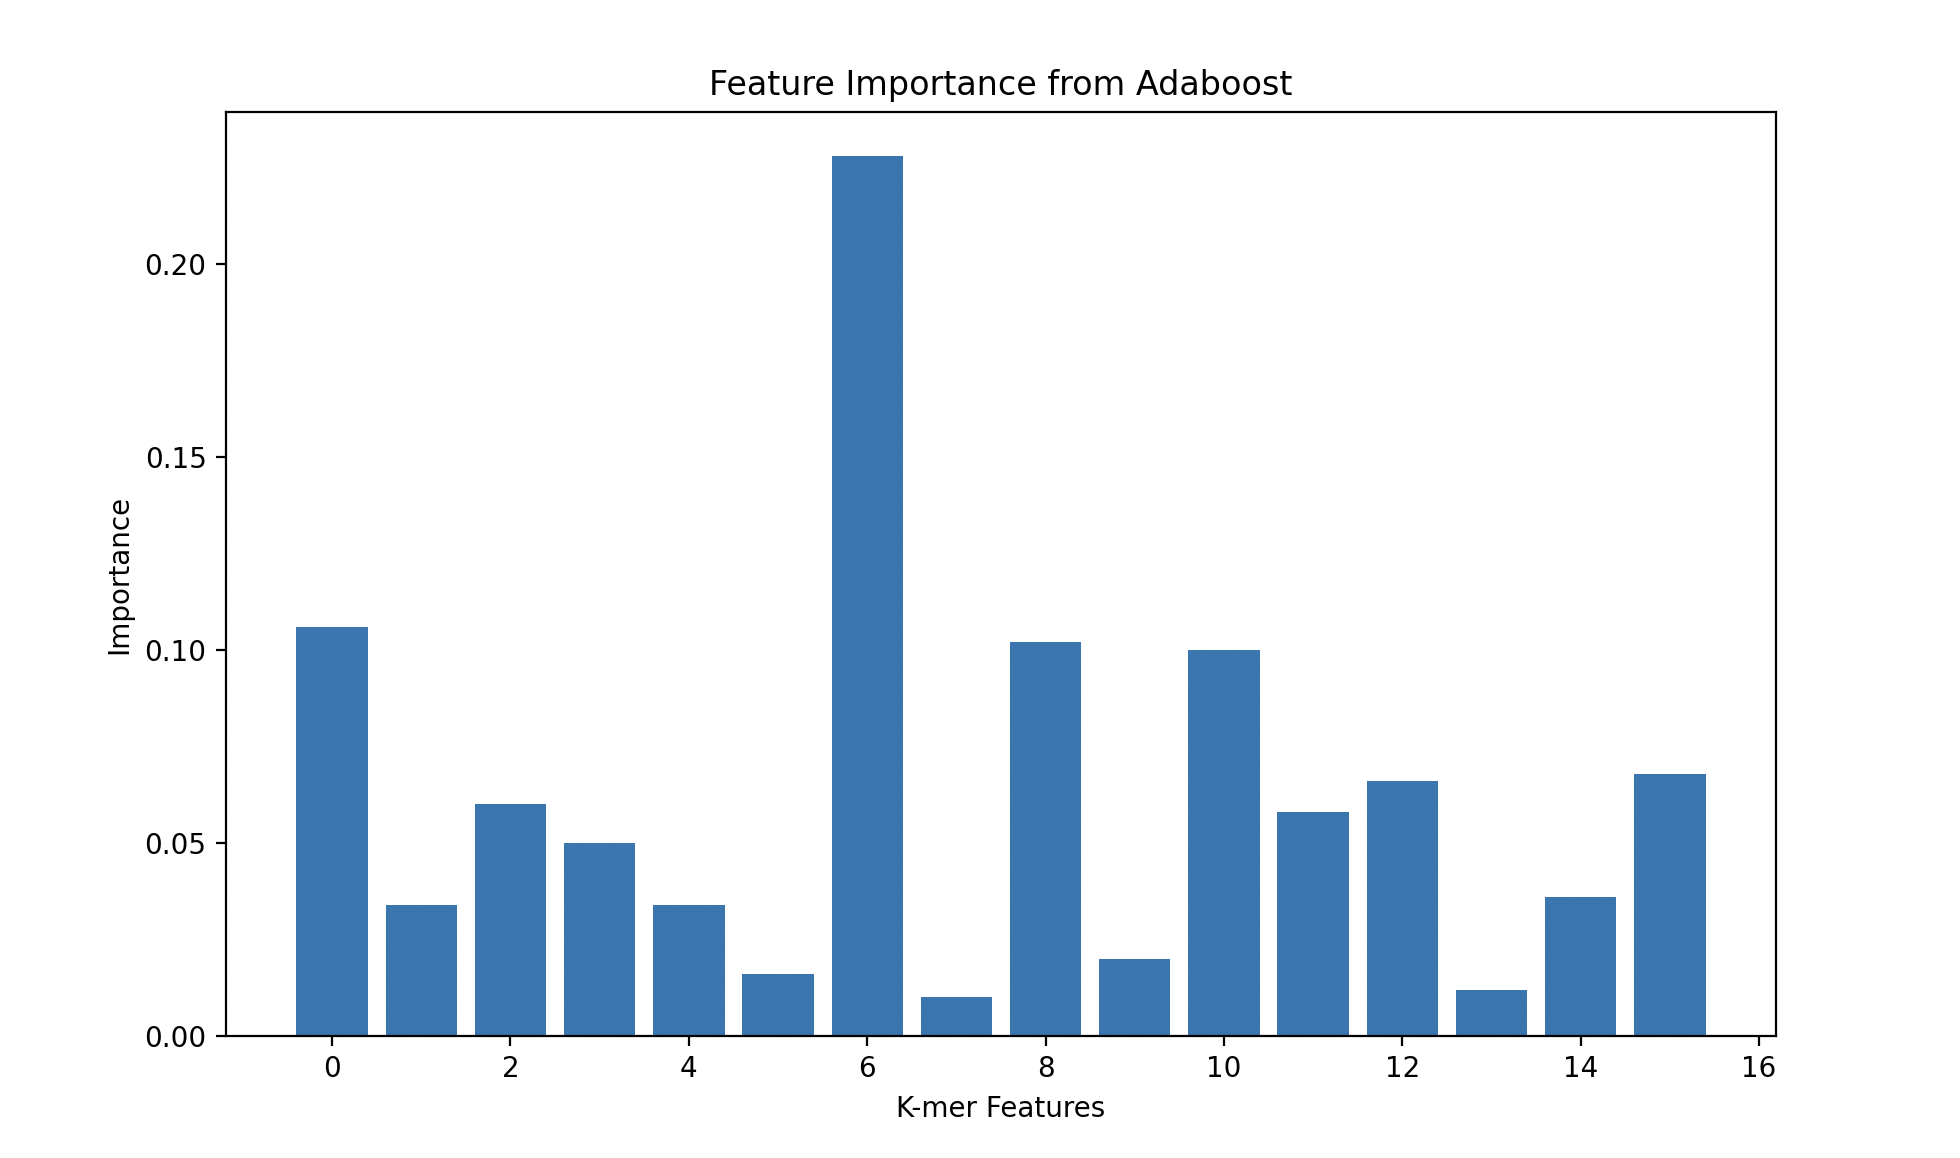
\includegraphics[height=0.67\linewidth]{Figures/AdaBoost_Feature.png}
        \caption*{(a) AdaBoost算法}
    \end{minipage}
    % \hfill % 添加空白填充,确保图片之间有一些间隔
    \begin{minipage}{0.49\linewidth}
        \centering
        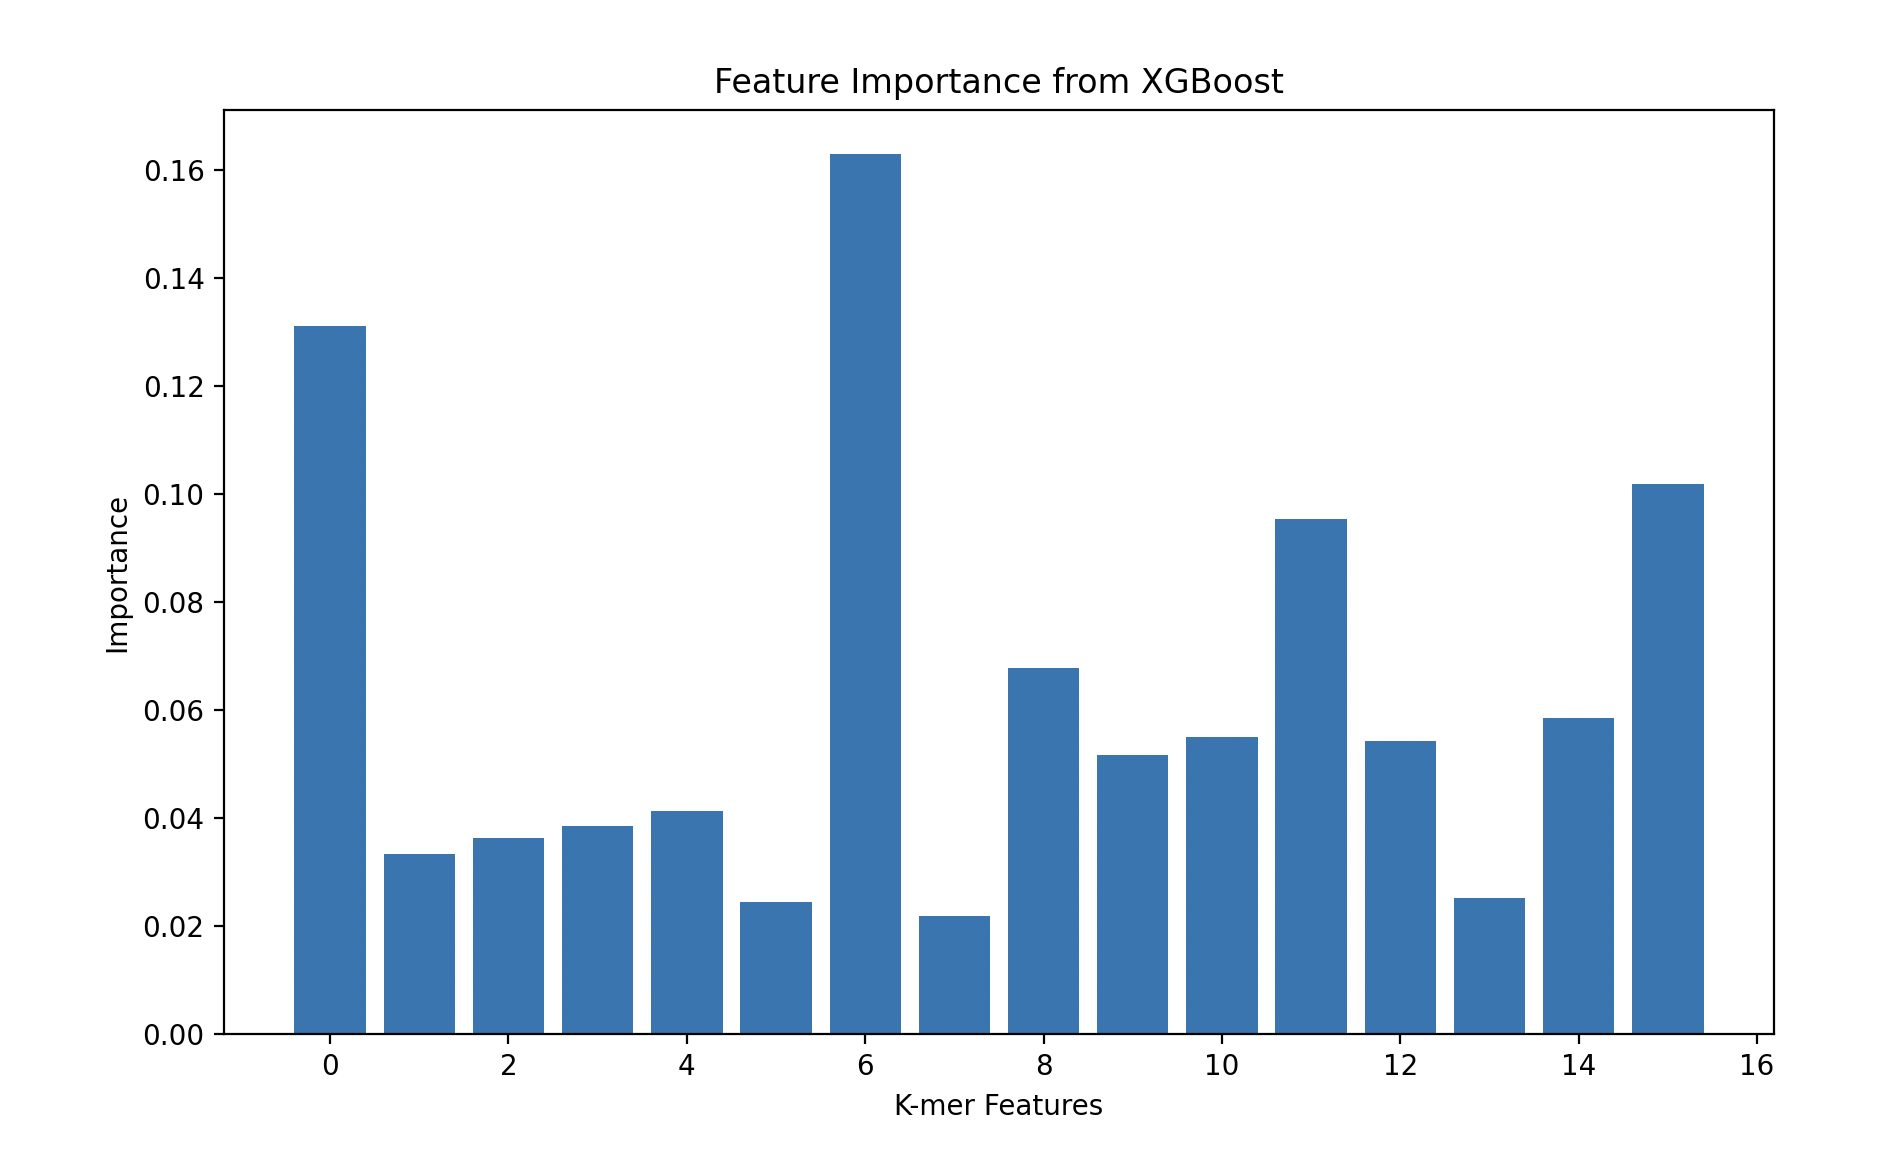
\includegraphics[height=0.67\linewidth]{Figures/XGBoost_Feature.png}
        \caption*{(b) XGBoost算法}
    \end{minipage}
    \caption{维度信息重要程度比较}
    \label{fig:维度信息重要程度比较}
\end{figure}

\textbf{在两个算法中第0,6,8,10,12,15种碱基对组合在分类中起到的效果最大,也即是对应的AA,CG,GA,GG,UA和UU碱基对组合出现的频率对RNA分类判断起到的作用最大。}同时,比较左右两图也可以发现在XGBoost算法中,权重的分配更为均衡,利用到了更多的特征信息;而AdaBoost算法中有个别碱基对组合的出现频率权重非常低,可能漏掉了这些特征提供的分类信息。这也从另一个侧面解释了XGBoost比AdaBoost算法的进一步提升。

\section{总结分析}
通过本次大作业的实践,我通过神经网络,支持向量机以及集成学习方法对RNA分类问题进行尝试,从测试集准确度的效果来说,几个方法之间总体差距不大,神经网络方法最好,支持向量机方法略显逊色。鲁棒性方面神经网络和XGBoost算法也展现出了一定优势。通过这一次的代码实践和上一次的课程作业,我对机器学习与知识发现课程后半学期的架构和内容有了更加深刻的理解。通过尝试对不同方法,一步步提升优化,也提升了我的代码实践能力,面对现实中的一些应用问题,我也能展现出更加多元的思路。

最后,再次感谢潘小勇和孙仕亮两位老师一学起来在机器学习与知识发现课程中的倾情授课,让我对机器学习和算法领域有了更加深刻的理解。




\section{附录}

\subsection{NN方法训练代码实现}

\begin{lstlisting}
def classification(training_file, test_file, k=3, hidden_size=128, batch_size=32, epochs=20, network='RNA_Classifier'):
    # 读取数据
    train_data = pd.read_csv(training_file)
    test_data = pd.read_csv(test_file)

    # 提取RNA序列和标签
    X_train = [kmer_encoding(seq, k) for seq in train_data.iloc[:, 2]]  # 3列为RNA序列
    y_train = train_data.iloc[:, 3].values  # 4列为标签
    
    X_test = [kmer_encoding(seq, k) for seq in test_data.iloc[:, 2]]
    y_test = test_data.iloc[:, 3].values
    
    # 转换为numpy数组
    X_train = np.array(X_train)
    X_test = np.array(X_test)

    # 标准化
    scaler = StandardScaler()
    X_train = scaler.fit_transform(X_train)
    X_test = scaler.transform(X_test)
    
    # 划分训练集和验证集
    # X_train, X_val, y_train, y_val = train_test_split(X_train, y_train, test_size=0.2, random_state=42)
    # 划分训练集和验证集,并保持标签分布一致
    X_train, X_val, y_train, y_val = train_test_split(X_train, y_train, test_size=0.2, random_state=42, stratify=y_train)
    
    # 转换为torch张量
    X_train_tensor = torch.tensor(X_train, dtype=torch.float32)
    y_train_tensor = torch.tensor(y_train, dtype=torch.float32).view(-1, 1)
    X_val_tensor = torch.tensor(X_val, dtype=torch.float32)
    y_val_tensor = torch.tensor(y_val, dtype=torch.float32).view(-1, 1)
    X_test_tensor = torch.tensor(X_test, dtype=torch.float32)
    y_test_tensor = torch.tensor(y_test, dtype=torch.float32).view(-1, 1)
    
    # 初始化神经网络
    input_size = X_train.shape[1]  # K-mer的数量(例如3-mer是64)
    if network == 'RNA_Classifier':
        model = RNA_Classifier(input_size, hidden_size)
    elif network == 'RNA_Classifier_2':
        model = RNA_Classifier_2(input_size, hidden_size)
    else:
        model = RNA_Classifier_3(input_size, hidden_size)
    
    # 损失函数和优化器
    criterion = nn.BCELoss()  # 二分类损失 交叉熵损失函数
    optimizer = torch.optim.Adam(model.parameters(), lr=0.0001)
    
    # 用于记录损失和准确率
    train_loss_history = []
    val_loss_history = []
    train_accuracy_history = []
    val_accuracy_history = []
    
    # 训练模型
    for epoch in range(epochs):
        model.train()
        running_loss = 0.0
        correct_train = 0
        total_train = 0
        
        for i in range(0, len(X_train), batch_size):
            # 获取一个batch的数据
            inputs = X_train_tensor[i:i+batch_size]
            labels = y_train_tensor[i:i+batch_size]
            
            # 前向传播
            outputs = model(inputs)
            loss = criterion(outputs, labels)
            
            # 反向传播和优化
            optimizer.zero_grad()
            loss.backward()
            optimizer.step()
            
            running_loss += loss.item()
            
            # 计算训练集准确率
            predicted = (outputs > 0.5).float()
            total_train += labels.size(0)
            correct_train += (predicted == labels).sum().item()

        # 计算训练集的平均损失和准确率
        train_loss = running_loss / len(X_train)
        train_accuracy = 100 * correct_train / total_train
        train_loss_history.append(train_loss)
        train_accuracy_history.append(train_accuracy)
        
        # 验证集评估
        model.eval()
        with torch.no_grad():
            val_outputs = model(X_val_tensor)
            val_loss = criterion(val_outputs, y_val_tensor).item()
            val_predicted = (val_outputs > 0.5).float()
            correct_val = (val_predicted == y_val_tensor).sum().item()
            total_val = y_val_tensor.size(0)
            val_accuracy = 100 * correct_val / total_val
            val_loss_history.append(val_loss)
            val_accuracy_history.append(val_accuracy)
        
        # 打印每个epoch的训练和验证集的损失和准确率
        if (epoch + 1) % 1 == 0:
            print(f"Epoch [{epoch+1}/{epochs}], "
                  f"Train Loss: {train_loss:.4f}, Train Accuracy: {train_accuracy:.2f}%, "
                  f"Val Loss: {val_loss:.4f}, Val Accuracy: {val_accuracy:.2f}%")
    
    # 测试模型
    model.eval()
    with torch.no_grad():
        y_pred = model(X_test_tensor)
        y_pred = (y_pred > 0.5).float()  # 二分类输出0或1
        
        accuracy = (y_pred == y_test_tensor).float().mean()
        print(f"Test Accuracy: {accuracy.item() * 100:.2f}%")
    
    # 绘制训练过程中的损失和准确率图
    epochs_range = range(1, epochs + 1)
    
    plt.figure(figsize=(12, 6))
    
    # 绘制损失
    plt.subplot(1, 2, 1)
    plt.plot(epochs_range, train_loss_history, label='Train Loss')
    plt.plot(epochs_range, val_loss_history, label='Validation Loss')
    plt.xlabel('Epochs')
    plt.ylabel('Loss')
    plt.legend()
    plt.title('Loss per Epoch')
    
    # 绘制准确率
    plt.subplot(1, 2, 2)
    plt.plot(epochs_range, train_accuracy_history, label='Train Accuracy')
    plt.plot(epochs_range, val_accuracy_history, label='Validation Accuracy')
    plt.xlabel('Epochs')
    plt.ylabel('Accuracy (%)')
    plt.legend()
    plt.title('Accuracy per Epoch')
    
    plt.tight_layout()
    plt.show()
    
    return model
    
\end{lstlisting}


\subsection{AdaBoost方法训练代码实现}
\begin{lstlisting}
def classification(training_file, test_file, k=3, n_estimators=50, learning_rate=1.0, max_depth=1):
    train_data = pd.read_csv(training_file)
    test_data = pd.read_csv(test_file)

    X_train = [kmer_encoding(seq, k) for seq in train_data.iloc[:, 2]]  # 第3列为RNA序列
    y_train = train_data.iloc[:, 3].values  # 第4列为标签
    
    X_test = [kmer_encoding(seq, k) for seq in test_data.iloc[:, 2]]
    y_test = test_data.iloc[:, 3].values

    X_train = np.array(X_train)
    X_test = np.array(X_test)

    scaler = StandardScaler()
    X_train = scaler.fit_transform(X_train)
    X_test = scaler.transform(X_test)

    X_train, X_val, y_train, y_val = train_test_split(X_train, y_train, test_size=0.2, random_state=42, stratify=y_train)

    base_estimator = DecisionTreeClassifier(max_depth=max_depth)

    model = AdaBoostClassifier(
        base_estimator=base_estimator,
        n_estimators=n_estimators,
        learning_rate=learning_rate,
        random_state=42
    )

    model.fit(X_train, y_train)

    y_val_pred = model.predict(X_val)
    val_accuracy = accuracy_score(y_val, y_val_pred)
    print(f"Validation Accuracy: {val_accuracy * 100:.2f}%")

    y_test_pred = model.predict(X_test)
    test_accuracy = accuracy_score(y_test, y_test_pred)
    print(f"Test Accuracy: {test_accuracy * 100:.2f}%")

    print("\nClassification Report (Test Set):")
    print(classification_report(y_test, y_test_pred))

    feature_importances = model.feature_importances_
    plt.figure(figsize=(10, 6))
    plt.bar(range(len(feature_importances)), feature_importances)
    plt.xlabel('K-mer Features')
    plt.ylabel('Importance')
    plt.title('Feature Importance from Adaboost')
    plt.show()
    return model
\end{lstlisting}




\subsection{XGBoost算法训练代码实现}
\begin{lstlisting}
def classification_with_xgboost(training_file, test_file, k=3, n_estimators=100, learning_rate=0.1, max_depth=3):
    train_data = pd.read_csv(training_file)
    test_data = pd.read_csv(test_file)

    X_train = [kmer_encoding(seq, k) for seq in train_data.iloc[:, 2]]  # 第3列为RNA序列
    y_train = train_data.iloc[:, 3].values  # 第4列为标签
    
    X_test = [kmer_encoding(seq, k) for seq in test_data.iloc[:, 2]]
    y_test = test_data.iloc[:, 3].values

    X_train = np.array(X_train)
    X_test = np.array(X_test)

    scaler = StandardScaler()
    X_train = scaler.fit_transform(X_train)
    X_test = scaler.transform(X_test)

    X_train, X_val, y_train, y_val = train_test_split(X_train, y_train, test_size=0.2, random_state=42, stratify=y_train)

    model = XGBClassifier(
        n_estimators=n_estimators,
        learning_rate=learning_rate,
        max_depth=max_depth,
        use_label_encoder=False,
        eval_metric='logloss',
        random_state=42
    )

    model.fit(X_train, y_train, eval_set=[(X_val, y_val)], early_stopping_rounds=10, verbose=True)

    y_val_pred = model.predict(X_val)
    val_accuracy = accuracy_score(y_val, y_val_pred)
    print(f"Validation Accuracy: {val_accuracy * 100:.2f}%")

    y_test_pred = model.predict(X_test)
    test_accuracy = accuracy_score(y_test, y_test_pred)
    print(f"Test Accuracy: {test_accuracy * 100:.2f}%")

    print("\nClassification Report (Test Set):")
    print(classification_report(y_test, y_test_pred))

    feature_importances = model.feature_importances_
    plt.figure(figsize=(10, 6))
    plt.bar(range(len(feature_importances)), feature_importances)
    plt.xlabel('K-mer Features')
    plt.ylabel('Importance')
    plt.title('Feature Importance from XGBoost')
    plt.show()
    return model
\end{lstlisting}


\end{document}